\documentclass[10pt,conference]{IEEEtran}
% http://networking2013.poly.edu/call-for-papers/paper-submission/
% Page limit 9 pages

\makeatletter
\def\ps@headings{%
\def\@oddhead{\mbox{}\scriptsize\rightmark \hfil \thepage}%
\def\@evenhead{\scriptsize\thepage \hfil \leftmark\mbox{}}%
\def\@oddfoot{}%
\def\@evenfoot{}}
\makeatother

\hyphenation{incoming}

\pagestyle{headings}

\usepackage[top=.75in, bottom=1in, left=.625in, right=.625in]{geometry}
\usepackage{graphicx}
%\usepackage[]{hyperref} %IEEE does not like hyperrefs...
\usepackage{breakurl}
\usepackage{url}
\usepackage[nocompress]{cite}
% \usepackage{verbatim}
% \usepackage{algpseudocode}
\usepackage{algpseudocode,algorithm}
% More customizeable version. Probably it would be better to convert pseudocode to 2e format
% \usepackage{algorithm2e} 
\usepackage{multirow}
\usepackage{times}
\usepackage{color}



\newfont{\nicettfont}{cmtt10}
\newcommand{\ndnName}[1]{``{\nicettfont #1}''}
\renewcommand{\texttt}[1]{{\nicettfont #1}}

\newcommand{\todo}[1]{\vspace{2 mm}\par \noindent \marginpar{\textsc{ToDo}}
\framebox{\begin{minipage}[c]{0.95 \columnwidth}
\tt #1 \end{minipage}}\vspace{5 mm}\par}
\graphicspath{{figures/}}

\begin{document}

\title{Interest Flooding Attack and Countermeasures in Named Data Networking}

% I PUT AUTHOR NAMES IN ALPHEBETICAL ORDER. It is the common practice in security and I always list authors alphebetically in my publications. -Ersin 
\author{
    \IEEEauthorblockN{Alexander Afanasyev\IEEEauthorrefmark{1}, Priya Mahadevan\IEEEauthorrefmark{2}, Ilya Moiseenko\IEEEauthorrefmark{1}, Ersin Uzun\IEEEauthorrefmark{2}, Lixia Zhang\IEEEauthorrefmark{1}}
    \IEEEauthorblockA{\IEEEauthorrefmark{1}University of California, Los Angeles
    \\\{afanasev, iliamo, lixia\}@cs.ucla.edu}
    \IEEEauthorblockA{\IEEEauthorrefmark{2}Palo Alto Research Center
    \\\{ersin.uzun, priya.mahadevan\}@parc.com}
}

\maketitle

\begin{abstract}
Distributed Denial of Service (DDoS) attacks are an ongoing problem in today's Internet, where packets from a large number of compromised hosts thwart the paths to the victim site and/or overload the victim machines. 
In a newly proposed future Internet architecture, Named Data Networking (NDN), end users request desired data by sending Interest packets, and the network delivers Data packets upon request only, effectively eliminating many existing DDoS attacks. 
However, an NDN network can be subject to a new type of DDoS attack, namely Interest packet flooding.  
In this paper we investigate effective solutions to mitigate Interest flooding.
We show that NDN's inherent properties of storing per packet state on each router and maintaining flow balance (i.e., one Interest packet retrieves at most one Data packet) provides the  basis for effective DDoS mitigation algorithms.
Our evaluation through simulations shows that the solution can quickly and effectively respond and mitigate Interest flooding.
\end{abstract}

\begin{IEEEkeywords}
Information-centric networks, named-data networking, denial-of-service
\end{IEEEkeywords}

\section{Introduction}
\label{sec:intro}

Named Data Networking (NDN)~\cite{ndn-conext, ndn-tr} is an ongoing research effort that aims to move the Internet into the future with a content-centric design that is capable of efficient content distribution and seamless mobility support. In contrast to today's Internet, a key goal of the NDN project is ``security by design." In fact, it goes a long way by guaranteeing the integrity and provenance of every Data packet with digital signatures and protecting user-privacy with no source addresses carried in the packets. However, one big question that is yet to be answered is: how does the NDN architecture fare in terms of its resilience against DDoS attacks? Especially since various forms of DDoS attacks pose a significant threat to the existing Internet infrastructure~\cite{arbor-report}, it is crucial to ensure that the new design is free of similar vulnerabilities.

NDN eliminates host-based addressing and makes data the first-class network entity. Instead of sending packets to a given IP address, NDN nodes request desired data by sending Interest packets carrying application-level data names, and the network returns the requested Data packets following the path of Interests. 
Such a shift automatically eliminates several long-standing DDoS attacks, including direct flooding and reflector attacks through source address spoofing~\cite{mirkovic2004taxonomy}.
%
However, malicious users can attack the network by sending an excessive number of Interests. 
Since each Interest consumes resources at intermediate routers as it is routed through the network, an excessive number of Interests can congest the network and exhaust a router's memory. 
We coin the term {\it Interest flooding} to refer to such attack and
this paper exclusively investigates the problem and the solution space for it. 

Our effort is an important first step towards a complete investigation of DDoS attacks in NDN. We experiment with three algorithms that allow routers to exploit their state information to thwart these attacks. Through extensive simulations, we show how one of our mitigation methodologies effectively shuts down malicious users while preventing legitimate users from service degradation. 
The rest of the paper is organized as follows. We provide an overview of NDN architecture in Section~\ref{sec:ccn-intro} and describe Interest flooding attacks in Section~\ref{sec:interest-flooding}. In Sections~\ref{sec:design} and \ref{sec:evaluation} we introduce techniques to mitigate these attacks, evaluate their effectiveness, and discuss their limitations. We summarize related work in Section~\ref{sec:related-work} . We discuss future work and conclude in Section~\ref{sec:conclusion}. 

\section{NDN Overview\label{sec:ccn-intro}}

In this section we briefly introduce NDN with a focus on its stateful forwarding plane (refer to \cite{ndn-conext, ndn-tr, adaptive-forwarding} for more details).
NDN is a receiver-driven, data-centric communication protocol.
All communications in NDN are performed using two distinct types of packets: \textit{Interest} and \textit{Data}. Both types of packets carry a \textit{name}, which uniquely identifies a piece of content that can be carried in one Data packet. Data names in NDN are hierarchically structured and an example name for the first segment of a youtube video would look like: \ndnName{/youtube/videos/0F8YdlkKO9A/0}.

To retrieve data, a consumer requests it by sending an Interest packet with the name of the desired content in it.
Routers use this name to route the Interest towards data sources, and a Data packet whose name matches the name in the Interest is returned to the consumer by following the reverse path of the Interest. Similar to IP, Interest forwarding is based on longest name prefix match, but, unlike IP, an Interest packet and its matching Data packet always take symmetric paths.
%% An Interest is ``satisfied'' when it is matched with a Data packet.

Each NDN router maintains three major data structures:
\begin{itemize}
\item \textit{Pending Interest Table (PIT)} holds all ``not yet satisfied'' Interests that have been sent upstream towards potential data sources. Each PIT entry contains one or multiple incoming and outgoing physical interfaces; multiple incoming interfaces indicate the same data is requested from multiple downstream users; multiple outgoing interfaces indicates the same Interest is forwarded along multiple paths.
\item \textit{Forwarding Interest Base (FIB)} maps name prefixes to one or multiple physical network interfaces, specifying directions where Interests can be forwarded. 
% Having one-to-many relationship in this table allows multipath forwarding of Interests.}
\item \textit{Content Store (CS)} temporarily buffers Data packets that pass through this node, allowing efficient data retrieval by different consumers.
\end{itemize}

When a router receives an Interest packet, it first checks whether there is a matching data in its CS.
If a match is found, the Data packet is sent back to the incoming interface of the Interest packet.
If not, the Interest name is checked against the entries in the PIT. 
If the name already exists in the PIT, then it can be a duplicate Interest (identified by a random number each Interest carries) that should be dropped,
or an Interest from another consumer asking for the same Data, which requires the incoming interface of this Interest to be added to the existing PIT entry.
If the name does not exist in the PIT, the Interest is added into the PIT and forwarded along the interface chosen by the strategy module, which uses FIB as input for its decisions.

When a Data packet is received, its name is used to look up the PIT.
If a matching PIT entry is found,
the router sends the Data packet to the interface(s) from which the Interest was received, caches the data in the CS, and removes the PIT entry.  Otherwise, the Data packet is deemed unsolicited and is discarded. 
Each Interest also has an associated lifetime; the PIT entry is removed when the lifetime expires.
Although the maximum lifetime is specified by users, it is ultimately a router's decision on how long it is willing to keep a PIT entry.  
For simplicity, we assume routers keep Interests in PIT for one second in our simulations.

\section{Interest Flooding Attacks in NDN}
\label{sec:interest-flooding}



As we explained earlier, Interest packets in NDN are routed through the network based on content name prefixes and consume memory resources at intermediate routers. This makes them a potential tool to launch DDoS attacks in NDN. An attacker or a set of distributed attackers can inject excessive number of Interests in an attempt to overload the network and cause service disruptions for legitimate users (Fig.~\ref{fig:flooding example}). 

\begin{figure}[htbp]
  \centering
  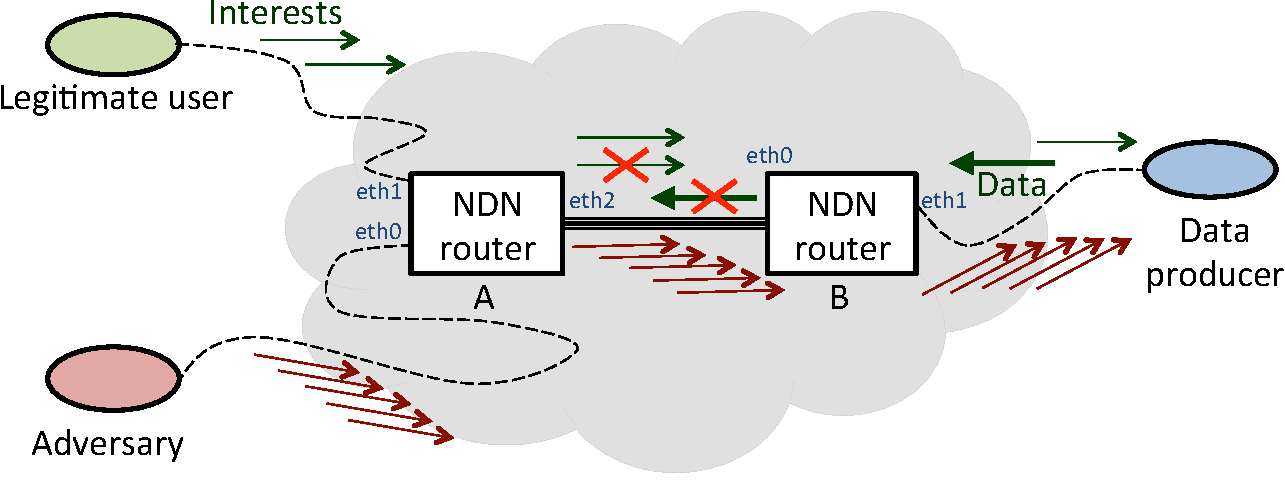
\includegraphics[scale=0.39]{attack-definition}
  \vspace{-0.6cm}
  \caption{Example of Interest flooding attack}
  \label{fig:flooding example}
\end{figure}


Since an NDN network fetches data by its name, an adversary cannot easily target specific routers or end-hosts.
However, an adversary can target a specific namespace.
For example in Fig.~\ref{fig:flooding example}, if the data producer is the exclusive owner of \ndnName{/foo/bar} namespace, both router B and the data producer would receive all Interests for \ndnName{/foo/bar/\ldots} that cannot be otherwise satisfied from in-network caches.
\footnote {This example assumes that the adversary floods the network with unique data names carrying \ndnName{\small /foo/bar} prefix to make them effective. It also assumes the producer is single-homed and the data is not replicated elsewhere. With multi-homed producers or replicated data, NDN would likely to cope better with DDoS attacks due its native multipath and adaptive forwarding~\cite{adaptive-forwarding} support.}
A large volume of such malicious Interests can disrupt service quality in NDN network in two ways: \emph{create network congestion} and \emph{exhaust resources on routers}.

Similar to packets in traditional networks, Interest packets in NDN consume a portion of network capacity. A large number of Interest packets might cause congestion and lead to legitimate packets being dropped in the network. In particular, a coordinated DDoS attack could target one specific namespace and concentrate attack traffic in certain segments of the network as routing in NDN is based on name prefixes. 


As NDN routers maintain per-packet states for each forwarded Interest (i.e., an entry in its PIT), an excessive amount of malicious Interests can lead to exhaustion of a router's memory, making the router unable to create new PIT entries for incoming Interests and disrupting service for legitimate users.

Nevertheless, creating an effective Interest flooding attack in NDN is non-trivial.
To efficaciously target a specific namespace (e.g., \ndnName{/newyorktimes/}), an adversary needs to make sure that (1) the expressed Interests are routed towards and as close to the data producer/provider as possible, and (2) new corresponding PIT entries are created for those interests and are stored at intermediate NDN routers for as long as possible. The former is achieved when interests share the same name prefix (e.g., \ndnName{/newyorktimes/}) and as long as they are not served from caches of intermediate routers---an interest is not forwarded upstream if a router can satisfy it from its content store. The latter requires every single malicious Interest to ask for a unique content---all Interests requesting the same content are collapsed to one PIT entry in routers. Thus, an adversary has to request either an unpopular (i.e., not cached in routers) or non-existing unique content with each Interest. Of the two options available to an adversary, the first one is challenging due to the difficulties around indexing content names in a particular namespace, coordinating a large number of bots to send unique Interests and sustaining the attack while the network is continuously caching the requested content objects. However, the second option {\it i.e.} requesting unique non-existing content with each Interest, is easy to achieve and sustain. An adversary can construct such Interests by concatenating a random name component to the victim namespace (e.g.,\ndnName{/newyorktimes/fgb...3rf3}) and can increase the memory usage at each router by lengthening the random component. In this paper, we exclusively focus on this particular attack strategy as it not only maximizes the damage from each malicious Interest but also is the one that is easy to launch and widely applicable to all namespaces (small or large). % other less effective strains of Interest flooding attacks can also be mitigated by applying the same or similar countermeasures described in the next section.  

In the rest of this paper, we use the general term \emph{Interest flooding attack} to refer to the above described attack and assume an attacker is limited to controlling a botnet of end-hosts only, i.e., we assume the routers in the network and the computers in the victim domain are not compromised.

%\paragraph{Assumptions} 
%E: These are assumptions for the simulations on hand and particulary to test for the worst case scenario in many aspects. They are not the paper's assumption and in fact the paper first should be more general on describing all possibilities. Then it should explain the assumptions for the simulations and discuss why they make sense and do NOT favor positive results in some way. 

% - assumptions about attacker position
% - assumptions about the producer / producer namespace
% - assumptions about the attack traffic / attack pattern

%In this paper we are making the following assumptions about the Interest flooding attack:
%\begin{itemize}
%\item only client nodes can be compromised and become attack bots;
%\item there are no colluding attackers inside the Data producer's network;
%\item the attack is carried only using unique junk Interests; and
%\item there is only one Data producer for the attacked prefix.
%\end{itemize}

%We also assume that NDN forwarding strategy uses only single-path Interest forwarding, always choosing the best-metric route advertised by the routing protocol.
%This way, we are able to analyze the attack in its best environment, as enabling the multi-path forwarding would only alleviate effects of the Interest flooding attack.

%In section~\ref{sec:discussion} we discuss potential of the Interest flooding attack under several other attack assumptions.

\section{Interest flooding mitigation methods}
\label{sec:design}

% Points what should be here:
% - What can be done (in general) to mitigate flooding attack
% - Which building blocks NDN architecture gives to mitigate Interest flooding attacks: Interest limits, ability to measure Interest satisfaction performance (Interest satisfaction stats)
% - Methods to set these limits: static/dynamic
% - Methods how limits can be applied: best-effort (fifo), "fair" queuing, probabilistic
% - Reference to caching: we don't consider it here, but caching provides additional level of protection, especially for certain types of attacks

% Our definition of attack mitigation is that good clients are still able to access data on the producer.

In this section we present several algorithms to mitigate Interest flooding attacks in NDN.  Our mitigation strategies feature varying degrees of implementation complexity and effectiveness---the higher the implementation complexity, the more effective is the algorithm against Interest flooding attacks. We start by describing our simple strategies and use the insights and lessons learned from the deployment of these to inform and design more effective mitigation techniques that work well in various topologies.

%   - Naive approach to Interest Limits (that is called physical limits everywhere else)
%     Example how this can be implemented in a simple way
%     Baseline solution
%   - Interest limits with "fair" queuing
%     Improving problem of simple limits (no single face can dominate), but doesn't solve the proble

% - Attack mitigation
%   - Per-incoming interface Interest statistics

%   - Dynamic Interests limit adjustments

%   - Probabilistic Interest accept

%The fact that each Data packet takes the reverse path of the corresponding Interest packet allows intermediate routers to match a received Data packet to the corresponding Interest packet and %thus determine which Interest packets were satisfied. As we describe in the rest of this section,  NDN routers can exploit this information to make informed decisions on which Interest packets to %forward, how many Interest packets to forward, and thus effectively defend against DDoS attacks.

%Our methods to mitigate Interest flooding attack rely on the fundamental principle of the NDN architecture: the flow balance between Interest and Data packets: one Interest packet (the only communication initiator) can be satisfied with at most one Data packet.
%Because NDN is host-to-host architecture (as opposed to end-to-end in the current IP Internet), the flow balance principle allow any entity on the network, end-hosts and routers, control what and how much Data they want to receive.
%Therefore, any node can limit the number of forwarded Interests, effectively limiting the amount of the retrieved Data.
%At the same time, each forwarded Interest can be used to build up various data plane performance statistics, such as per-incoming interface ratios of satisfied Interests.

%\subsection{Na\"{i}ve attack mitigation}

%We start with a couple of naive strategies that can be used to migitate attacks in an NDN network and describe the pitfalls associated with these strategies.

% In a normal network operation, the size of Interests packets is supposed to be significantly smaller than the size of the requested Data.

% All communication in NDN network is host-to-host and receiver-driven.

An obvious and na\"ive solution to defend against Interest flooding attacks is to restrict the number of Interests forwarded through the network. To this end, we exploit a 
 fundamental principle of NDN architecture---flow balance between Interest and Data packets. Flow balance refers to the fact that one Interest can be satisfied by at most one Data packet. This principle allows intermediate routers to control the inbound data traffic by controlling the number of outstanding Interests in the network. 
One simple implementation technique  is for an NDN router to limit the number of forwarded Interests out of each interface based on the physical capacity of the corresponding interface. This technique is a slight modification of the well-known {\it Token Bucket} algorithm that is currently widely used in packet-switched networks. Analogous to the {\it Token Bucket} algorithm, NDN routers keep track of the amount of data requested that can fully utilize the downstream link (estimated from the number of forwarded Interests) and once the link capacity limit has been reached, they no longer forward new incoming Interests. Ideally, the number of tokens (the pending \emph{Interest Limit}) for each link will be proportional to the link's bandwidth-delay product (BDP)~\cite{tcp-survey}. We can formalize this value as follows:
% With the objective to request as many Data packets, as downstream link can pump through, we are getting the following equation for Interest limit:
%
\begin{equation}
\label{eq:interest limit}
\small \mathrm{Interest\ Limit} = Delay\ [s] \cdot \frac{\mathrm{Bandwidth\ [Bytes/s]}}{\mathrm{Data\ packet\ size\ [Bytes]}}
\end{equation}

In the above equation, \emph{Delay} is the expected time for the Interest to be satisfied and \emph{Data packet size} is the size of the returning Data packet.
Although both these values are not known a priori, it is not really necessary to use their exact values.
One can simply set the pending Interest limit based on the average values of round trip time and observed Data packet size, as network buffers can smooth out most of the network fluctuations.

This {\it Token Bucket} approach might be exceptionally restrictive in forwarding Interests---not all Interests will result in a Data packet---and might result in underutilization of the network. However, the biggest drawback of this algorithm is the fact that it can nourish DDoS attacks. If a router has utilized all its tokens to forward malicious Interests, it can no longer forward incoming Interests from legitimate users till the pending malicious Interests start to expire. One way to get around this issue is to impose a per interface limit, so that malicious Interests are not allowed to entirely consume the limits of a specific interface. We describe this technique in greater detail below.

%That is, if it is known that the amount of already requested data ($=$~amount of forwarded Interests) can fully utilize the downstream link, an NDN node---either an end-user or an NDN router---has absolutely no point in forwarding new incoming Interests and creating corresponding PIT entries.
%For example, if a router A on Fig.~\ref{fig:flooding example} already forwarded 125 Interests requesting 1000-byte Data packets, any new incoming Interests can be almost safely dropped, provided the link capacity between A--B is 100~Mbps and delay is 10~ms.
%In other words, 125 Data packets returned by router B will fully utilize the link ($125 \times 1000 \mathrm{~bytes} \approx 10\mathrm{~ms} \times 100\mathrm{~Mbps}$) and any excess Data would be dropped.
%
%\subsubsection{\textbf{Interest limits (physical limits)}}
%\label{sec:physical limits}
%
%\subsection{Physical limits}
\label{sec:physical limits}

The requirement to send an Interest in order to receive Data packet, provides an NDN consumer a unique opportunity to request the right amount of Data.
Moreover, the same opportunity to control the amount of data flow is given not only to consumers, but all routers between consumer and producer (or nearby caches).  
In other words, every node, either a consumer or an intermediate router, is able to control how much data it wants to receive by limiting the number of forwarded Interests.

The limitation can implemented in a number of different ways, including leaky bucket scheduling and window-based flow control.
We decided to following TCP-like window-based flow control and applied the sliding window approach to implement Interest limits.

The size of the window defines how many Interests can be send out before Interests get satisfied or expired.
From the one hand, this size should be large enough to ``fill the pipe,'' meaning that a node needs to send enough Interests to receive Data at full capacity of the incoming link.
On the other hand, the window's size should not be too large to avoid excessive buffering and congestion of the Data packet.
Thus, the ideal size for such a window need to be defined proportional to link's bandwidth-delay product~\cite{tcp-survey}.
With the objective to request as many Data packets, as downstream link can pump through, we are getting the following equation for Interest limit:

\[
\mathrm{Interest\ Limit} = Delay\ [s] \cdot \frac{\mathrm{Bandwidth\ [Bytes/s]}}{\mathrm{Data\ packet\ size\ [Bytes]}}
\]

Note that the value of \textit{Delay} is not known a priory and varies between different Interest-Data flows.
However, we do not need to know the exact value of the delay and can set it as an average round trip delay among all flows (with a reasonable filtering of outliers).
This way, the statistical traffic multiplexing with link-level buffering will allow full utilization of the downstream link.
Exactly the same reasoning can be applied to the \textit{Data packet size} parameter, which can also be set to an average observed Data packet size.

Unlike rate-based approaches, window-based limiting does not require precise knowledge about the rate, as well does not need precise scheduling mechanisms.
Like in TCP, the window-based flow is self-clocking, easily adjusting itself to any traffic patterns.

%%% Local Variables: 
%%% mode: latex
%%% TeX-master: "../paper"
%%% End: 


%%%%%%%%%%%%%%%%%%%%%%%
%%%%%%%%%%%%%%%%%%%%%%%
%%%%%%%%%%%%%%%%%%%%%%%

\subsubsection{\textbf{Token bucket with per interface fairness}}
\label{sec:queuing}

To address the lack of fairness associated with the na\"ive {\it Token Bucket} approach, we modify it to ensure that the Interests forwarded by a router on each interface represent a fair mix of Interests received from neighboring nodes. For example, in Fig.~\ref{fig:flooding example} router A can ensure that the tokens associated with Interests sent out on interface {\texttt eth2}  are fairly distributed across incoming interfaces \texttt{eth0} and \texttt{eth1}. 
%Due to the expected small volume of Interests, we cannot merely rely on network buffers to perform statistical multiplexing of Interests, as they would almost never be %buffered.
%At the same time, until bag of tokens is not empty, there is no reason to delay Interest forwarding, as we do not known how many and from which interfaces Interests %will arrive in the future.
In order to achieve our goal of ensuring ``fair'' mixing of Interests from all neighboring nodes, 
%, we implement an additional features to support buffering of Interests, if they cannot be immediately forwarded. 
we extend the Pending Interest Table to support flagging of Interests that cannot be immediately forwarded and implement hierarchical queues for each interface (see Fig.~\ref{fig:queueing}). 
This mechanism is essentially a class based queuing~\cite{floyd1995link}, with classes for each outgoing and incoming interface.
%As an alternative to hierarchical queues, one can also use an approach based on virtual time. For details, please see ~\cite{zhang1990virtual}.
We note that unlike normal queuing, Interest queues do not actually store a packet, but merely a bi-directional pointer to the existing PIT entry.
Thus, a PIT entry can be quickly updated when the Interest is actually forwarded, and the element can be easily removed from the queue when the Interest expires.

%For the buffering part, we can reuse Pending Interest Table, with a small extension to support flagging of the Interests that cannot be forwarded immediately (see example on Fig.~\ref{fig:queueing}). 
%As for the mixing part, we need an additional fair queuing mechanism, which can be implemented in a form of hierarchical queues (on Fig.~\ref{fig:queueing})\footnote{This essentially is a class based queuing, with classes for each outgoing/incoming interface.} or using virtual time approach~\cite{zhang1990virtual}. 

\begin{figure}[thb]
  \centering
  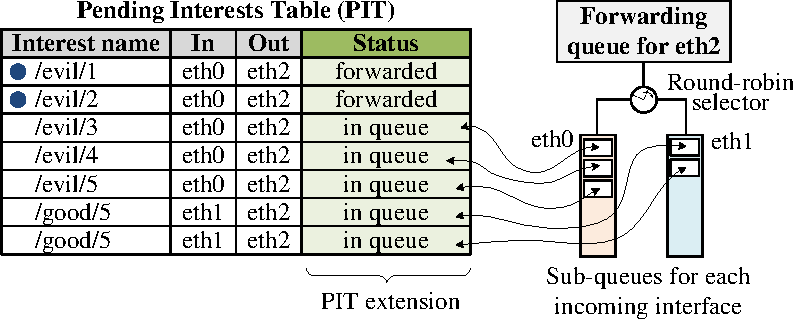
\includegraphics[scale=0.6]{queue}
  \vspace{-0.4cm}
  \caption{Interest queuing: if tokens are unavailable, the router creates a PIT entry, but instead of forwarding, it enqueues the Interest}
  \label{fig:queueing}
\end{figure}

We present a formalized description of this algorithm in Pseudocode~\ref{alg:queuing}. 
By setting appropriate queue sizes, we can control the amount of physical resources utilized at a router.
 % (such as memory and computation power). 
It is also important to set a sensible value for how long an Interest can be enqueued. 
If an Interest is enqueued for a long time, by the time it is dequeued and forwarded, the retrieved Data packet might be dropped at the downstream routers if their corresponding state expired. 
For our evaluations, we empirically chose to enqueue Interests up to 10\% of their original lifetime.
% We believe that implementing additional mechanisms on each pair of communicating routers to keep the Interests from getting stale would mitigate this issue, though the details are beyond the scope of this paper.
% Alex: I don't believe there is a need for separate discussion about "freshness", as we already introduced concept of lifetime
% {\color{red} \it Priya:  We need to  touch upon the Interest freshness issue in the NDN overview section; else we should get rid of this bit.}

%It should be noted that enqueued Interests should not be kept in the queue for a prolonged period of time.
%Otherwise, by the time the Interests reaches the Data, the state could have been long expired downstream, effectively making such an Interest useless.
%Additional mechanisms of pair-wise agreements between NDN routers and periodic Interest refresh can solve this particular problem, but it is out of the scope of the present paper.

%The algorithm extends the base Physical limits algorithm by enabling queuing when the bag of tokens is empty (lines 7--10), as well as by triggering an action (lines 16--21), when a token becomes available and enqueued Interest can be finally forwarded.
%At the same time, the algorithm limits number of Interests allowed in a queue, constraining memory usage increase by at most a constant factor, compared to the base Physical limits algorithm (i.e., memory attack on routers are still unfeasible). 


\floatname{algorithm}{\small Pseudocode}

%%%%%%%%%%%%%%%%%%%%%%%%%%%%%%
%%%%%%%%%%%%%%%%%%%%%%%%%%%%%%
%%%%%%%%%%%%%%%%%%%%%%%%%%%%%%

\begin{algorithm}[h]
\footnotesize
\caption{\small Token bucket with per interface fairness}
\label{alg:queuing}
\begin{algorithmic}[1]
\For{\textbf{each} interface \textbf{if}}
    \State{$L_{if} \leftarrow$ Interest Limit according to (1)}
    \State{$O_{if} \leftarrow 0$} \Comment{Outstanding Interests on interface \textbf{if}}
\EndFor

\vspace{0.1cm}

\Function{OutInterest}{Interest \textbf{i}, InInterface \textbf{in}, OutInterface \textbf{out}}
    \If{$L_{out} - O_{out} > 0$} \Comment{\textbf{out} is under limit cap}
        \State $O_{out} \leftarrow O_{out} + 1$  \Comment{``borrow'' a token from the bucket}
        \State add \textbf{out} to PIT entry and forward \textbf{i} to \textbf{out}
    \Else
        \State Queue $q \leftarrow out$.GetSubQueue($in$)
        \If{$Size(q) < L_{out}$}
           \State $q$.PushInterest($i$)
           \State add \textbf{out} to PIT entry, and link PIT entry with the queue
        \Else
           \State drop Interest
        \EndIf
    \EndIf
\EndFunction

\vspace{0.1cm}

\State{} \Comment{\textit{Whenever $L_{out} - O_{out}$ becomes larger than zero}}
\Function{TokenBecomesAvailable}{}
    \State Queue $q \leftarrow$ $out$.GetRoundRobinSubQueue 
    \State Interest $i \leftarrow$ $q$.PopInterest
    \State update PIT entry and Forward($i$, $out$)
\EndFunction

\vspace{0.1cm}

\Function{InData}{Data \textbf{d}}
   \State lookup PIT entry \textbf{p} for data \textbf{d}
   \For{\textbf{each} outgoing interface \textbf{out} in \textbf{p}}
        \State $O_{out} \leftarrow O_{out} - 1$ \Comment{``return'' token}
   \EndFor
\EndFunction

\vspace{0.1cm}

\Function{Timeout}{PIT entry $p$}
   \For{\textbf{each} outgoing interface \textbf{out} in \textbf{p}}
        \State $O_{out} \leftarrow O_{out} - 1$ \Comment{``return'' token}
   \EndFor
\EndFunction


\end{algorithmic}
\end{algorithm}


As we show in Section~\ref{sec:evaluation}, this algorithm provides partial relief from Interest flooding attacks, allowing legitimate users to successfully fetch Data for 15--20\% of their expressed Interests. 
We note that while this algorithm might be reasonable for ensuring limited fairness in an NDN network, it is ineffective in protecting legitimate users from malicious ones. 
Attackers are able to successfully thwart access to content for legitimate users by sending a relatively modest volume of malicious Interests.


%At the same time, the Physical limits with or without fair queueing allows attackers to send a relatively small volume of Interests in order to significantly impact service for the legitimate users.
%Therefore, to successfully solve the problem, we need a fundamentally different, more intelligent approach, allowing localization of the attack traffic as close as possible to the attack origin.


%%%%%%%%%%%%%%%%%%%%%%%
%%%%%%%%%%%%%%%%%%%%%%%
%%%%%%%%%%%%%%%%%%%%%%%

The key drawback of the {\it Token bucket with per interface fairness} algorithm is that it still admits a relatively large number of Interests from malicious users. A considerable percentage of these malicious Interests are forwarded all the way to content producers, thereby reducing resources available to serve legitimate users.  This algorithm attempts to ensure that each interface does not forward more than its fair share of Interests, but in doing so, it drops both legitimate and malicious Interests. For any strategy to be effective in defending against Interest flooding attacks, it must be able to detect and differentiate malicious requests from legitimate ones. 
% `Good' Interests from legitimate users must be admited and forwarded appropriately. 
Thus, the key question is how can we devise mitigation algorithms that allow a router to distinguish between `good' and `bad' Interests? 

%One can try a black- or whitelisting approach. However, besides the fact that source black- and whitelisting cannot work in %NDN as it does not feature source addresses, it requires extraneous knowledge to classify the incoming Interests.

%Priya: I have added the below point specifically to point out that a router cannot determine from the prefix name alone whether /parc is good  or bad...
  
%{\color{red} \textbf{Alex: This paragraph is confusing to me. I would remove it.} In NDN one cannot easily distinguish a `good' prefix from a `bad' one. Content producers must be able to support %dynamic generation of Data packets to satisfy incoming Interest packets---thus, an Interest that cannot be satisfied by matching Data from any intermediate router's cache is necessarily forwarded %to the producer for possible dynamic Data packet generation. 
%Thus intermediate routers cannot determine if the prefix is `good' or `bad' based on the prefix name alone---DDoS mitigation techniques that rely on whitelisting or blacklisting of certain %namespaces  will be inefficient and likely ineffective. }

% Alex: I'm not sure that this part is relevant... The point I see is that blacklisting and whitelisting is not 100% effective, but it can be used in both worlds

% In today's host-based Internet architecture where DDoS mitigation techniques rely on blacklisting of ``dark'' IP prefixes or whitelisting of good IP prefixes.
% Unlike IP, in NDN one cannot easily distinguish a `good' prefix from a `bad' one. 
% Content producers must be able to support dynamic generation of Data packets to satisfy incoming Interest packets---thus, an Interest that cannot be satisfied by matching Data from any intermediate router's cache is necessarily forwarded to the producer for possible dynamic Data packet generation. 
% Thus intermediate routers cannot determine if the prefix is `good' or `bad' based on the name alone---DDoS mitigation techniques that rely on whitelisting or blacklisting of certain namespaces  will be inefficient and likely ineffective. 


\subsection{Intelligent attack mitigation}
\label{sec:intelligent mitigating}

%While the Interest limit is the key building block to suppress mechanisms of the Interest flooding attack, legitimate Interests need to be somehow prioritized and malicious Interests need to be somehow penalized in order to completely suppress the attack.
%That is, instead of processing Interests always based on the first-in-first-serve rule, NDN routers need some basis to treat the incoming Interests differently.
%Thus, the primary task in bringing intelligence to the Interest flooding attack mitigation is to proactively distinguish between legitimate and malicious Interests.

In order to distinguish between legitimate and malicious Interests, we leverage another unique feature of  NDN architecture---guaranteed symmetric flow of Interest and Data packets. Since a Data packet takes the reverse path of the corresponding Interest packet, a router is guaranteed to see if an Interest it forwarded resulted in a matching Data packet or timed out. %The only exception being if Interest/Data packets were lost along the way due to congestion in the network.
Since malicious Interests are not likely to bring data back (as discussed in Section~\ref{sec:interest-flooding}), this information can be utilized by routers in differentiating attack and legitimate traffic.  %Therefore, intermediate routers can classify the ones that brings data back as legitimate, while the ones that timed out can be marked as malicious.\footnote{Recall that in order to maximize effect of the Interest flooding attack, an adversary expresses a large volume of junk Interests (see Section~\ref{sec:interest-flooding}).}  
%Implications of other types of attacks are discussed in Section~\ref{sec:discussion}.}

This timeout-based differentiation method is reactive in nature: one cannot determine in advance if an Interest will result in a timeout or Data being retrieved. However, routers can proactively maintain up-to-date statistics of Interest satisfaction ratios (number of forwarded versus number of satisfied Interests), and use this statistic to determine whether an incoming Interest should be forwarded or dropped. For example, maintaining independent Interest satisfaction ratio statistics for each incoming interface is sufficient to reasonably predict whether an Interest received from a neighbor connected to this interface will result in a Data packet or a timeout if forwarded. Statistics can also be kept at finer granularities such as per outgoing interface, per name prefix, etc. that can further improve the estimates. A router's goal should be to prioritize Interests that bring Data back while quickly penalizing those that occupy resources but don't result in a returning Data packet. In order to allow negative statistics to build up fast and positive statistics to  deteriorate quickly, we use the standard exponentially weighted moving average, performed once a second with $\alpha$ coefficient $e^{-1/30}$, approximately corresponding to a 30-second averaging window.

%Choosing the right balance between these contradictory requirements is a challenge and we explore this topic further  in the evaluation section.  %{\color{red} \it Priya: we should address the one that works best such as exponentially weighted moving average in eval section - it doesn't belong %here.} 

%The devil is always in the details.
%From the one hand, such statistics needs to start penalizing adversaries as soon as possible (i.e., negative stats should build up fast).
%On the other hand, the positive statistics should not deteriorate too fast (i.e., positive stats should be relatively long-term).
%Our preliminary experiments showed that the standard exponentially weighted moving average, performed once a second with $\alpha$ coefficient $e^{-1/30}$, approximately corresponding to a 30-second averaging window, provides a good balance between the two contradictory requirements.

% \subsubsection{\textbf{Data plane performance tracking}}
% \label{sec:stats}

% Note that there is a condition (line 6 in Pseudocode~\ref{alg:probabilistic model}) to check if there is a valid statistics point.
% This condition is extremely important, because it first provides a basis to distinguish between known facts (i.e., good or bad satisfaction ratio for the incoming interface) and unknown facts (e.g., the first time an Interests arrives on the interfaces).
% Second, it gives an opportunity to recover from a bad history (history of unsatisfied Interests) after malicious Interests are ceased to flow in.
% Essentially, this recovery relies on statistics module to perform time-based invalidation of historical data (timely, but not too quickly\footnote{Otherwise, attackers may send short bursts of malicious Interests, successfully avoiding differential Interest treatment}).


Pseudocode~\ref{algo:interest stats} formally defines how statistics can be generated for  each incoming interface. Note that in order to ensure decaying of relative statistics (e.g., ratio between the number of unsatisfied and forwarded Interests), only unsatisfied statistics needs to be exponentially smoothed (lines 23--26).  

\floatname{algorithm}{\small Pseudocode}

%%%%%%%%%%%%%%%%%%%%%%%%%%%%%%
%%%%%%%%%%%%%%%%%%%%%%%%%%%%%%
%%%%%%%%%%%%%%%%%%%%%%%%%%%%%%

\begin{algorithm}[h]
\footnotesize
\caption{\small Interest satisfaction statistics}
\label{algo:interest stats}
\begin{algorithmic}[1]

\For{\textbf{each} interface \textbf{if}}
    \State $F_{if} \leftarrow 0$ \Comment{forwarded Interests from interface \textbf{if}}
    \State $\hat F_{if} \leftarrow 0$ \Comment{averaged value of $F_{if}$}

    \State $U_{if} \leftarrow 0$ \Comment{unsatisfied Interests from interface \textbf{if}}
    \State $\hat U_{if} \leftarrow 0$ \Comment{averaged value of $U_{if}$}
\EndFor

\vspace{0.1cm}
\Function{OutInterest}{Interest \textbf{i}, InInterface \textbf{in}}
  \State $F_{in} \leftarrow F_{in} + 1$
  \State record \textbf{\emph{in}} in the list of incoming interfaces for \textbf{\emph{i}}
\EndFunction

\vspace{0.1cm}
\Function{InterestTimeout}{Interest \textbf{i}}
    \State lookup the list of incoming interfaces for \textbf{\emph{i}}

    \For{\textbf{each} interface \textbf{if} in the list}
        \State $U_{if} \leftarrow U_{if} + 1$
    \EndFor
\EndFunction

\vspace{0.1cm}

\State {} \Comment{\textit{Exponentially weighted moving average smoothing}}
\Function{EWMA}{} \Comment{Every second}
\State $\alpha \leftarrow e^{-1.0/30.0}$  %\Comment{$\approx$ 30~sec average}

\For{\textbf{each} interface \textbf{if}}
    \State $\hat U_{if} \leftarrow \alpha \cdot \hat U_{if} + (1 - \alpha) \cdot U_{if}$ 
    \State $U_{if} \leftarrow 0$ 

    \If{$F_{if} > 0$} \Comment{To ensure decaying of ratio $U_{if}/F_{if}$}
        \State $\hat F_{if} \leftarrow \alpha \cdot \hat F_{if} + (1 - \alpha) \cdot I_{if}$ 
        \State $F_{if} \leftarrow 0$ \Comment{Reset counters}
    \EndIf
\EndFor

\EndFunction

\end{algorithmic}
\end{algorithm}


Fig.~\ref{fig:ratio example} illustrates the resulting dynamics of the statistic during and after an Interest flooding attack. The attack duration is from 10 to 70~seconds. Prior to start of the attack, the percentage of unsatisfied Interests is zero.  
The statistics build up rapidly as soon as Interests start to time out, which happens approximately one second after the start of the attack.
%\footnote{Again, we are assuming that Interests are admitted for a maximum period one second.}
For the duration of the attack (10--70~seconds), the percentage of unsatisfied Interests is close to 100\%: 
when the ratio is close to 100\%, routers drop all incoming Interests, resulting in decaying of the statistics until a new Interest is admitted, which eventually brings statistics back near 100\% point.
Finally, the ratio exponentially decays after the attack ceases.

\begin{figure}[htbp]
  \centering
  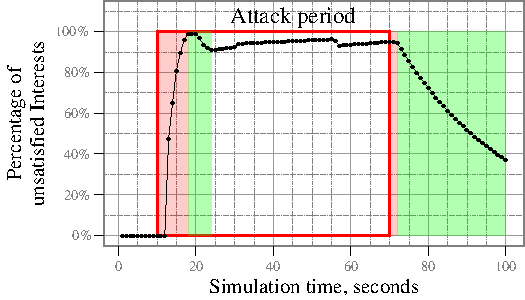
\includegraphics[scale=0.8]{limits}
  \vspace{-0.3cm}
  \caption{Dynamics of  unsatisfied Interests statistics on a gateway's interface towards the attacker}
  \label{fig:ratio example}
\end{figure}

%%%%%%%%%%%%%%%%%%%%%%%
%%%%%%%%%%%%%%%%%%%%%%%
%%%%%%%%%%%%%%%%%%%%%%%

\subsubsection{\textbf{Satisfaction-based Interest acceptance}}
\label{sec:probabilistic}

Having successfully implemented a technique to gather statistics on Interest satisfaction ratios, our next challenge is in using these ratios to penalize malicious Interests. A straightforward method to achieve this enforcement is to use the Interest satisfaction ratio as a direct probability for accepting (forwarding) or rejecting an incoming Interest (see Pseudocode~\ref{alg:probabilistic model}).
%Apart from the Interest satisfaction statistics generation, there is a question how this statistics can be used to actually enforce prioritization and penalizing of Interests.


\floatname{algorithm}{\small Pseudocode}

%%%%%%%%%%%%%%%%%%%%%%%%%%%%%%
%%%%%%%%%%%%%%%%%%%%%%%%%%%%%%
%%%%%%%%%%%%%%%%%%%%%%%%%%%%%%

\begin{algorithm}[h]
\footnotesize
\caption{\small Satisfaction-based Interest acceptance}
\label{alg:probabilistic model}
\begin{algorithmic}[1]
\State{} \Comment{Same init, InData and Timeout functions as in Pseudocode~\ref{alg:queuing}}

\vspace{0.1cm}
\Function{OutInterest}{Interest \textbf{i}, InInterface \textbf{in}, OutInterface \textbf{out}}

    \State{} \Comment{Use uniform probability distribution model $P(X)$}
    \State{} \Comment{$P(X) : \forall x \in [0,1] \Rightarrow P(x) = x$}
    
    \If{$F_{in} > \theta $} \Comment{At least some Interests were forwarded before}
        \State $s \leftarrow (1 - U_{in} / F_{in})$
        \State Drop interest with probability $P(s)$
    \EndIf

    \State{forward the Interest, subjecting to token bucket limits}
\EndFunction

\end{algorithmic}
\end{algorithm}

Parameter $\theta$ on line 5 of Pseudocode~\ref{alg:probabilistic model} ensures that the probabilistic model is not enforced when the volume of Interests arriving at a particular interface is small. This step is critical to provide an opportunity for legitimate users to regain their share of resources after temporary Data delivery failures.

A drawback of the satisfaction-based Interest acceptance method is that each router on the path makes an independent decision on whether to forward or drop an Interest. 
As a result of these independent decisions,  the probability of legitimate Interests being forwarded decreases rapidly as the number of hops between the content requester and producer grows; worsening the Interest satisfaction statistics and resulting in further drops.
In our example in Fig.~\ref{fig:flooding example}, the router A observes 50\% satisfaction rate for \texttt{eth1} and 0\% rate for \texttt{eth0}. 
At the same time, router B observes a 30\% satisfaction rate for its \texttt{eth0} interface.
Next time a legitimate Interest arrives at router A, it has a 50\% chance of being forwarded further, and if forwarded, it has only a $50\% \times 30\% = 15\%$ probability of being forwarded further towards the data producer. With each increasing hop in the network, the probability of being forwarded to the next hop decreases significantly. 
One way to prevent this overreaction and unfair penalization is to ensure that the decision taken at each router on whether to forward or drop the Interest is not independent of the decision taken at preceding routers. An explicit notification such as a gossip protocol between neighboring NDN routers might alleviate the problem, but we leave the design and evaluation of it to future work.
%{\color{red}Alex: we should state that it is out of scope of the paper to evaluate this issue}

%%%%%%%%%%%%%%%%%%%%%%%
%%%%%%%%%%%%%%%%%%%%%%%
%%%%%%%%%%%%%%%%%%%%%%%

\subsubsection{\textbf{Satisfaction-based pushback}}
\label{sec:dynamic limits}

% Differential treatment of Interests received from different interfaces can be achieved in a more elegant way, without reverting to probabilistic methods.

The previous algorithm---the satisfaction-based Interest acceptance---divides the available forwarding tokens among all interfaces in proportion to their Interest satisfaction ratios.
% Given the drawbacks of this algorithm, the same effect can be achieved without relying on probabilistic models. 
An alternate algorithm for proportional token distribution without overreaction is to enable and enforce explicit Interest limit for each incoming interface, where the value of the limit depends directly on the interface's Interest satisfaction ratio.
Routers need to announce these limits to their downstream neighbors, ensuring that any Interest forwarded from the downstream router is allowed to get through, resulting in genuine Interest satisfaction statistics.

The formal definition of the satisfaction-based pushback algorithm is presented in Pseudocode~\ref{alg:dynamic limits}, while Fig.~\ref{fig:dynamic limits example} illustrates how the algorithm will work in our example in Fig.~\ref{fig:flooding example}.
Assuming an initial token bucket limit $L=10$ and the current satisfaction ratio for router A is 50\% for \texttt{eth1} and 0\% for \texttt{eth0}, and for router B the ratio is 30\% for \texttt{eth0}, each node will set and announce the following  incoming interface limit $L'$: 
\begin{enumerate}
\item router B will set and announce the incoming interface limit $L'=3$;
\item router A, after receiving announcement from B will readjust its incoming interface limits to $L'_{eth1} = 1.5$ and $L'_{eth0} = 0$; and
\item both legitimate users and adversaries may either obey or ignore the announced limit, which will in any case be enforced by router A.
\end{enumerate}


\begin{figure}[htbp]
  \centering
  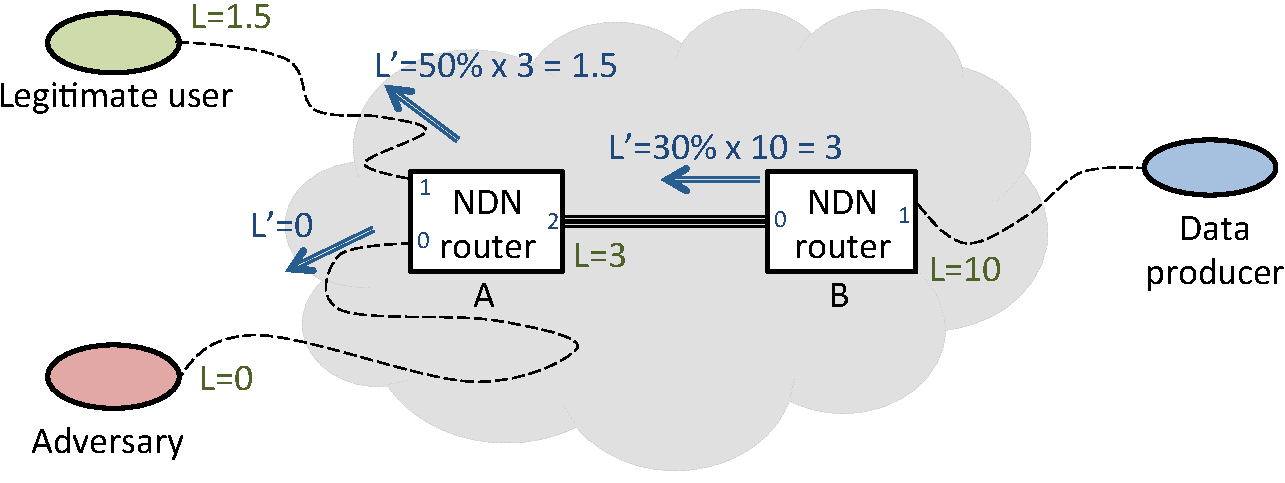
\includegraphics[scale=0.3]{dynamic-limits}
  \vspace{-0.3cm}
  \caption{Satisfaction-based pushback example
%: routers explicitly tell neighbors how many Interest packets they can deliver to the Data producer%
}
  \label{fig:dynamic limits example}
\end{figure}


\floatname{algorithm}{\small Pseudocode}

%%%%%%%%%%%%%%%%%%%%%%%%%%%%%%
%%%%%%%%%%%%%%%%%%%%%%%%%%%%%%
%%%%%%%%%%%%%%%%%%%%%%%%%%%%%%
{ 
\begin{algorithm}[h]
\footnotesize
\caption{\small Satisfaction-based pushback}
\label{alg:dynamic limits}
\begin{algorithmic}[1]
% \State{}\Comment{Same initialization, InData and Timeout functions as in Pseudocode~\ref{alg:queuing}}
\State{} \Comment{Same init, InData and Timeout functions as in Pseudocode~\ref{alg:queuing}}
\vspace{0.1cm}
\State{$\forall f \in \mathrm{interfaces} : L'_{f} \leftarrow L_{f}$} \Comment{Per-incoming interface Interest limit} 

\vspace{0.1cm}

\State{} \Comment{\textit{Announcement from the neighbor}}
\Function{InLimits}{InInterface $in$, Limit $L'$}
    \State $L_{in} \leftarrow L'$
\EndFunction

\vspace{0.1cm}

\Function{AnnounceLimits}{} \Comment{\textit{E.g., every second}}
\For{\textbf{each} outgoing interface $out$}

   \For{\textbf{each} incoming interface $in$}
        \State $L'_{in}= {L_{out}} \times (1 - U_{in}/F_{in})$
        \State AnnounceLimit($in$, $L'_{in}$)
   \EndFor

\EndFor
\EndFunction

\end{algorithmic}
\end{algorithm}


The zero limit for the adversary's link implies that  router A is temporarily not willing to accept any Interests from this interface until the statistics decay to an appropriate level (recall Fig.~\ref{fig:ratio example}).
At the next iteration of the satisfaction-based pushback algorithm, a legitimate user will be able to gradually improve the statistics on both routers A and B as all Interests from the user will get through and return Data, eventually resulting in a full allowance ($L'=L=10$) in the links between the routers A and B, and the user and router A.

We note that while in the description of the satisfaction-based pushback algorithm we explicitly used ``outgoing'' and ``incoming'' interfaces,  all interfaces can be both incoming and outgoing.
Thus, it may not be entirely clear which outgoing limit $L_{out}$ (line 10 in the algorithm) should be used to calculate the incoming limit $L_{in}$.
To overcome this problem, in our actual implementation we enforced separate incoming/outgoing interface limits for each individual FIB entry.
That is, for each FIB entry we set a separate Interest limit for each incoming interface (${L'}_{in}^{fib}$) based on the sum of FIB entry limits for each outgoing interface $L=\sum{L_{out}^{fib}}$.


Both satisfaction-based Interest acceptance and satisfaction-based pushback algorithms are forms of a well-known push-back mechanism~\cite{Pushback}, but with several core differences. 
First, we are suppressing (pushing back) unwanted requests for data, not actual data itself.
Second, differentiating between good and bad Interests is based on the traffic symmetry principle of NDN.
% Alex: I'm not entirely sure about this point... 
Finally, both intelligent attack mitigation algorithms can be deployed at all times without degrading network performance even when there are no active attackers. 


\section{Evaluation of Interest flooding mitigation methods}
\label{sec:evaluation}

% List all possible parameters, say clearly which ones we vary, and which ones we do not, along with explanations.

% Metrics that we will consider in our evaluation (Satisfaction rate for good clients, Link utilization near producers, 

% alex: what's a point of latency?  it would matter only for queueing method and we not really pushing this method
% Latency for good clients, good versus bad interests as a function of time

In this section, we present an in-depth evaluation study, aiming to quantify the effectiveness of all our Interest flooding attack mitigation methods.
We used the open-source ndnSIM~\cite{ndnsim} package, which implements NDN protocol stack for NS-3 network simulator (\url{http://www.nsnam.org/}), to run simulations for a variety of network topologies and scenarios. 
We extended ndnSIM with our three mitigation algorithms---token bucket with per interface fairness, satisfaction-based Interest acceptance, and satisfaction-based pushback---and evaluated the effectiveness of each algorithm independently.

% For evaluating the effectiveness of each mitigation algorithm, every router in the simulated topology runs the mitigation algorithm under study.

% why we chose small scale topology
% what point we wanted to show we small scale
% what points we wanted to verify with larger-scale internet like topology

% Metrics
% not sure if i already explained that. our essential qualitative metric is .  
% To quantify the effectiveness of the mitigation mechanism this  metric we use satisfaction percentages of user Interests.

The metric we choose to quantify the effectiveness of our algorithms is the {\it percentage of satisfied Interests for legitimate users}. This metric corresponds to the quality of service experienced by legitimate users when the network is under attack. In other words, if the network implements a mitigation method $X$ and a high percentage of user-expressed Interests are satisfied even while the network is under attack, then one can conclude that method $X$ is highly effective at mitigating the attack.% We also ensure that all Interests expressed by legitimate users during a period of no-attack are satisfied.
 
%Quality of the attack mitigation methods directly corresponds to the quality of service for the legitimate users during an ongoing attack, which in NDN network can be quantified through percentage of satisfied Interest.
%For example, if the network implements a mitigation method $X$ and under the attack majority of user-expressed Interests are getting satisfied, then the method $X$ can be seen as highly effective.
%At the same time, if only a small percentage of the expressed Interest are getting satisfied during the attack, the method $X$ can be called ineffective. 

% Traffic pattern
In our experiments, we assumed that legitimate users express Interests at constant average rates with randomized time gap between two consecutive Interests, where the random number for the gap follows a uniform distribution. We believe that this traffic pattern provides a reasonable approximation of traffic mix from all network users without excessive buffering. To quantify the behavior of our mitigation strategies under a worst-case attack scenario, we assumed that all the attackers send junk Interests as fast as they can. Further, no Interest---including legitimate ones---can be satisfied from caches.  We also configured routers for single-path Interest forwarding and there is only one single-homed producer for the prefix under attack.
%(remember, that Interest limits will not allow real flooding of Intersests in all of the designed mitigation algorithms).

% Alex: not sure how to argue about the traffic pattern
%Although this pattern may seem not truly realistic, it approximates a good statistical mix of traffic from all network users without excessive network buffering.

%In addition to that, in each run of the simulation we ensure that all Interests expressed by the legitimate users during a no-attack period are satisfied.
%For simplicity, we also equalized the average rates with which the legitimate users express Interests.
%At the same time, the attackers are sending junk Interests as much as they can get through (remember, that Interest limits will not allow real f%looding of Intersests in all of the designed mitigation algorithms).

We ran our simulations on two different network topologies---a smaller binary tree topology and a much larger ISP-like topology. We use a binary tree topology as it represents one of the worst cases to defend against Interest flooding DDoS attacks. The larger ISP topology reflects how our mitigation methods would perform when deployed on the real Internet.
Again, to study the performance of our mitigation strategies under a range of conditions, we varied the percentage of attackers in the network---the values ranged from 6\% attackers to over 50\% attackers in the network.
% Fixed parameters
We set the \emph{delay} and \emph{data size} parameters for the Interest limit calculation (formula \ref{eq:interest limit}) to a fixed 
value for every node in the simulated topology. In particular, for the small-scale binary tree topology, we set delay to 80~ms, while for the large-scale ISP topology we set it to 330~ms (the order of the largest RTT). The data size is 1100~bytes for all simulation runs and topologies.
% THIS IS BULLSHIT! There is absolutely no logic to set the delay to the same value on all nodes in the network. We discussed multiple times that you should fix it so that the delays are realistic and gets smaller as the nodes gets closer to the producer...


%%%%%%%%%%%%%%%%%%%%%%%%%%%%%%%%%%%%%%%%%%%%%%%%%%
%%%%%%%%%%%%%%%%%%%%%%%%%%%%%%%%%%%%%%%%%%%%%%%%%%

\subsection{Small-scale evaluations}
\label{sec:small-scale}

% Topology description
%To assess baseline quality of the designed Interest flooding attack mitigation methods, we evaluated them first using a %simplistic small-scale binary tree topology 
In Fig.~\ref{fig:small-scale}, we depict the binary-tree topology that we used for our initial experiments.
Legitimate users as well as attackers were placed on leaf nodes (top row of red nodes) as shown in the figure. There are 16 end users (both legitimate and attackers) in this topology, each expressing Interests that are routed towards a single data producer, placed at the root of the tree.  Each link in this topology is assigned a bandwidth of 10~Mbps and a randomized propagation delay ranging from 1 to 10 ms. 

% Alex: should we mention that?
%The main reason to chose a binary tree topology was that it represents one of the worst cases to defend against flooding DDoS %attacks.
%That is, sharing of the network links exponentially increases as decreasing level of the binary tree.

\begin{figure}[]
  \centering
  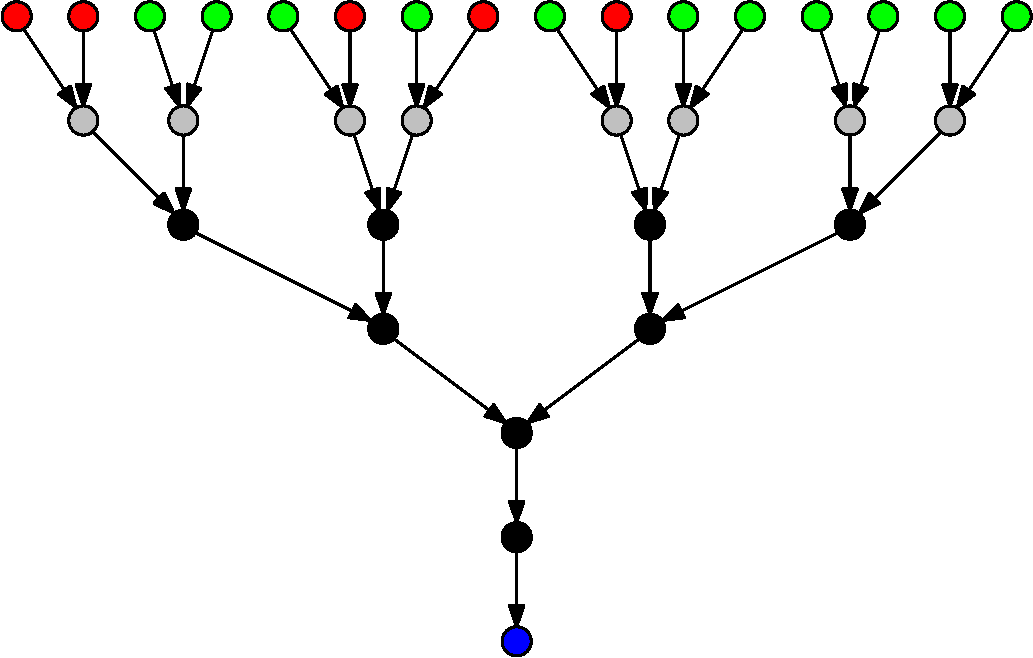
\includegraphics[scale=0.2]{topo-tree-evil-5-good-0-producer-gw}
  \caption{Small-scale binary tree topology}
  \label{fig:small-scale}
\end{figure}

% in 10 independent runs of each simulation, where we randomized position of the adversaries along the legitimate users.   In all runs, the total number of legitimate and malicious uses were fixed, meaning that when we increase number of attackers, we decrease the number of legitimate users.   

\subsubsection{Effectiveness of the three mitigation algorithms}

%The first set of experiments aims to evaluate reaction of the network and Interest flooding attack mitigation methods mechanisms under a moderate-level DDoS attack.
%For this purpose, we simulated four different network scenarios, in which all routers implements the same attack mitigation algorithm, either token bucket with per interface fairness, satisfaction-based Interest acceptance, or satisfaction-based pushback (Section~\ref{sec:design}).

Our goal is to compare the effectiveness of each mitigation method and quantify the percentage of Interests satisfied for all legitimate users while the network is under attack. For each mitigation algorithm, we perform 10 independent simulation runs, where we randomly choose 7 client nodes to represent adversaries while the remaining 9 client nodes represent legitimate users. In each run we simulate a 10-minute attack window (total simulation time was 30 minutes, with attack starting at the 10-minute mark). We plot the minimum and maximum range for observed Interest satisfaction percentages for all legitimate users aggregated across the 10 simulation runs as a function of time for each mitigation algorithm in Fig.~\ref{fig:small-scale attack progress}. Token bucket with per-interface fair queuing performs the worst, while satisfaction-based pushback performs the best, with almost a 100\%  satisfied Interests for all legitimate users.

%A short and simplistic summary of the results is that the first two attack mitigation methods do not work at all, and the last two are working quite good.

\begin{figure}[]
  \centering
  \hspace{-0.8cm}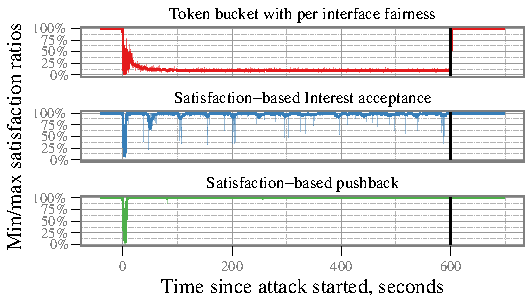
\includegraphics[scale=0.8]{paper-topo-tree/tree-good-0-producer-gw}
  \vspace{-.3cm}
  \caption{Interest satisfaction ratio as a function of time for binary-tree topology with 7 attackers and 9 legitimate users}
  \label{fig:small-scale attack progress}
  \vspace{-.4cm}
\end{figure}

%\paragraph{\textbf{Simple token bucket}}

%{\color{red}Alex: should this discussion be removed or we still want to keep it (as it is referenced later and potentially before)}

%Let us take a deeper look on what is happening with the simple token bucket algorithm.
%Essentially, we observe an extremely successful denial of service attack, where attackers almost completely shut down legitimate users from the Data producer (using a relatively small amount of Interests, as token bucket restricts the number of forwarded Intersets!).
%This ``success'' can be explained using a simplistic example, illustrated on Fig.~\ref{fig:three router example}, where each router has only one token for Interest forwarding.
%In this example we assume that both the legitimate user and the adversary send Interests in about the same time.
%
%\begin{figure}[t]
%  \centering
%  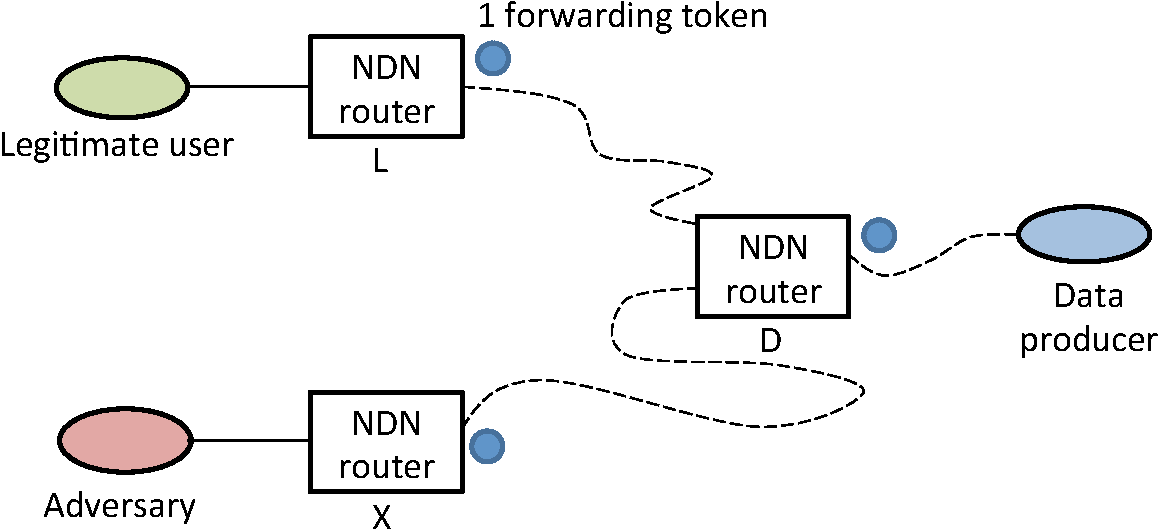
\includegraphics[scale=0.3]{physical-limits-sync-problem}
%  \caption{Three-router topology, with one legitimate and one malicious user}
%  \label{fig:three router example}
%\end{figure}
%
%Both router L and router X will forward the Interests, as both of them have a free token available.
%At router A, two cases are possible, either of Interests can arrive first, resulting in a quite different effects.
%When legitimate Interest arrives first, then there are no problem. 
%Router A will capture the token, forward the Interest, which will be quickly satisfied, releasing the token for future uses.
%In the mean time, malicious Interest will be dropped at router A, and router X will release the hold for the token in one second (i.e., after the maximum time Interests are admitted), enabling a new round of competition for router A's resources.
%
%In the case when malicious Interest is sent a little bit earlier, then router A will forward malicious Interests, dropping a legitimate one, and causing ``lock out'' for one second.
%In the instant when the token gets released at router X, an adversary is able to push new Interest towards router A, which may arrive in the exact time A's token gets released (assuming an idealistic environment).
%As a result, the adversary recaptures router A's token and extends the ``lock out'' for another second, denying service to the legitimate user without sending any massive numbers of Interests.

\paragraph{\textbf{Token bucket with per interface fairness}}

We observe a successful DDoS attack, where 40\% attackers succeed in significantly shutting down the remaining 60\% legitimate users---a mere 15\% of their Interests are satisfied by Data from the producer. Contrary to expectations, the 60\% legitimate users do not receive at least 60\% of network resources. As described in the previous section, the key limitation of this algorithm is that it still admits Interests from attackers and causes congestion and packet drops near the victim. %Significantly reducing the number of accepted malicious Interests is fundamental for improving the effectiveness of any mitigation algorithm. 

%The described problem arises from the clocking effect and can be solved in a number different ways.
%Augmenting token bucket algorithms with per-interface fair queueing allows us to eliminate the clocking effect. 
%That is, in the second case when router A releases the token after the first ``lock out'' period, it will immediately process previously enqueued Interests from the legitimate user.
%However, because the Interest time out (``lock out'' time) is most likely be larger than the time to actually fetch the Data, an adversary is still able to ``unfairly'' deny service to good guys.
%Ideally, if there are only 40\% of compromised users, the rest good users should get at least 60\% of network resources, which is not true as can be seen on Fig.~\ref{fig:small-scale attack progress}.
%We expect that reducing the maximum hold time for Interests (e.g., to an order of average RTT) would improve overall performance for legitimate users, with negative effect of requiring extra complexity for Intersets processing.

\paragraph{\textbf{Satisfaction-based Interest acceptance}}

The effectiveness of this algorithm stems from the fact that routers can differentiate and limit malicious Interests into the network%, thereby ensuring availability of network resources for serving legitimate users
. The observed periodic dips in the Interest satisfaction ratios of legitimate users in Fig.~\ref{fig:small-scale attack progress} is a direct result of Interest satisfaction rate statistics decaying with time. The 50-second period approximately corresponds to the selected exponential decaying parameter $\alpha=e^{−1.0/30.0}$, which decays statistics to $1/e$ of the initial value within 30~seconds and to $\approx$20\% within 50~seconds.
 % that ranges from 30~seconds to 50~seconds. 
%The primary reason that such minimum peaks exist is the fact that 
When Interests from attackers start to get readmitted, they cause degradation of statistics on routers close to the producer (i.e., routers that observe mixed traffic from legitimate and malicious users). Consequently, this degradation reduces the probability of legitimate Interests getting through (see Section~\ref{sec:probabilistic}) until malicious Interests are ``pushed back'' again to the edge.

%When routers more intelligently process incoming Interests (i.e., based on the incoming interface statistics), the Interest flooding attack becomes virtually ineffective.
%That is, malicious Interests are simply not getting admitted to the network, not being able to create much service disturbance for the legitimate users.

\paragraph{\textbf{Satisfaction-based pushback}}

In our simulations, this mitigation algorithm was able to effectively shut down attackers and ensure almost all the Interests from legitimate users are satisfied. 
%The only potential problem with the satisfaction-based pushback algorithm is that it features 
We observe a  sharp dip in the satisfaction ratio curve at the start of the attack as it takes a few seconds for all routers to be fully aware of the attack. However, recovery is quick as malicious Interests start to time out and explicit Interest limit announcements start to succeed in containing malicious Interests close to the attacker. Till then, the network, for a short period of time (under 10~seconds for all simulation runs), fails to provide 100\% service for legitimate users. Once the malicious Interests are effectively shut down, all Interests from legitimate users are satisfied. Unlike the satisfaction-based Interest acceptance scenario, we do not observe any periodic dips in the satisfaction curve, as the pushback algorithm effectively guarantees that once an Interest is admitted, it will likely be routed all the way to the data producer.

\subsubsection{Network reaction to varying number of attackers}

Our next goal is to study the effectiveness of our mitigation algorithms as a function of increasing adversaries in the network.
To this end, we vary the percentage of attackers in the topology from 6\% to over 50\%. Since the total number of end users in the topology is constant, as the number of attackers increases, the number of legitimate users decreases. All other parameters and experimental setup are consistent with the previous experiment. As before, for each mitigation algorithm, we perform 10 independent simulation runs.
%The second set of conducted experiments was aimed to answer the question of the effect and quality of the Interest flooding attack mitigation algorithm under different attack volume.
%To do this, for each algorithm we varied the number of adversary nodes in the topology, keeping the total number of client nodes constant: 1 attacker and 15 legitimate users, 3 attackers and 13 legitimate users, etc.

%Since at this point the overall attack dynamics of all the attack mitigation algorithms is relatively clear, 
% In other words, each point captured in the box plot graph corresponds to 1-second averaged satisfaction ratio for a user in an individual simulation run.

\begin{figure}[htbp]
  \centering
  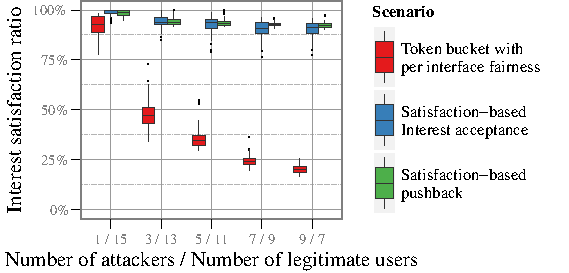
\includegraphics[scale=0.8]{paper-topo-tree/tree-good-0-producer-gw-avg-1-min}
  \vspace{-.3cm}
  \caption{Average Interest satisfaction ratios for the first minute of the experiment as a function of increasing attackers in the network}\vspace{-.1cm}
  \label{fig:small-scale-topo boxplot}
\end{figure}

In Fig.\ref{fig:small-scale-topo boxplot} we present  the Interest satisfaction ratio for legitimate users aggregated over the 10 simulation runs for the first minute of the attack. The results are as expected---for all three mitigation algorithms, as the percentage of attackers in the network increases, the lower is the Interest satisfaction ratio for legitimate users.
In the case of token bucket with per-interface fairness algorithm, just 3 attackers can halve the quality of service for the remaining 13 legitimate users. While the two intelligent attack mitigation algorithms also show a decline in service quality as the percentage of attackers increases, this decline is much more gradual and marginal. In the case of satisfaction-based pushback algorithm, during the first minute of the attack over 90\% of Interests from legitimate users are satisfied even if 50\% of end nodes are malicious.  
 


% \begin{figure}[htbp]
%   \centering
%   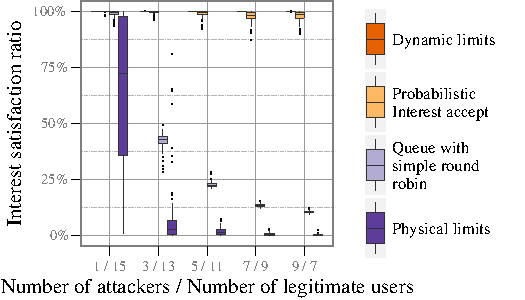
\includegraphics[scale=0.9]{tree-topo-var-evils-max-consumers-30mins/tree-good-0-producer-gw-avg-1-min-after-1-min}
%   \caption{Average consumer Interest satisfaction ratios (second minute)}
%   \label{fig:small-scale-topo 2}
% \end{figure}

%%%%%%%%%%%%%%%%%%%%%%%%%%%%%%%%%%%%%%%%%%%
%%%%%%%%%%%%%%%%%%%%%%%%%%%%%%%%%%%%%%%%%%%

\subsection{Large scale simulations}
\label{sec:largescale}

%To check validity of the small-scale experiment results, we performed a larger-scale evaluation based on a modified version of 

In this section, we investigate the behavior of our mitigation strategies under a more realistic, large-scale network topology. The ISP topology we used is based on a modified version of Rocketfuel's AT\&T topology~\cite{rocketfuel}.
%In order to approximate the general structure of the Internet,
% (scale-free structure, customer-provider, and peer-to-peer relations)
We extract the largest connected component comprising of 562 nodes from this original topology and separate the nodes into three categories: clients, gateways, and backbones. Nodes having degree less than four are classified as clients (344 red nodes as shown in Fig.~\ref{fig:large-scale}), nodes directly connected to clients are classified as gateways (109 green nodes), and the remaining nodes are classified as backbones (109 blue nodes). 
%(To ensure that paths in the topology are ``valley-free,'' we augmented the topology with necessary backbone-to-backbone links.) 
We assign bandwidth and  delay values to links based on their type---both values are random numbers within the respective ranges as shown in Table~\ref{tab:large-scale}. We experiment with placing the data producer at both a gateway node as well as backbone node, which we randomly pick for each simulation run. Similar to the binary tree topology experiments, we fix the number of malicious nodes at approximately 40\% (140 out of 344 client nodes in the topology) and randomly pick these nodes for each simulation run. We conduct 10 simulation runs for each mitigation algorithm, with the attack duration spanning a 5-minute interval.

\begin{figure}[htbp]
  \centering
  \vspace{-.1cm}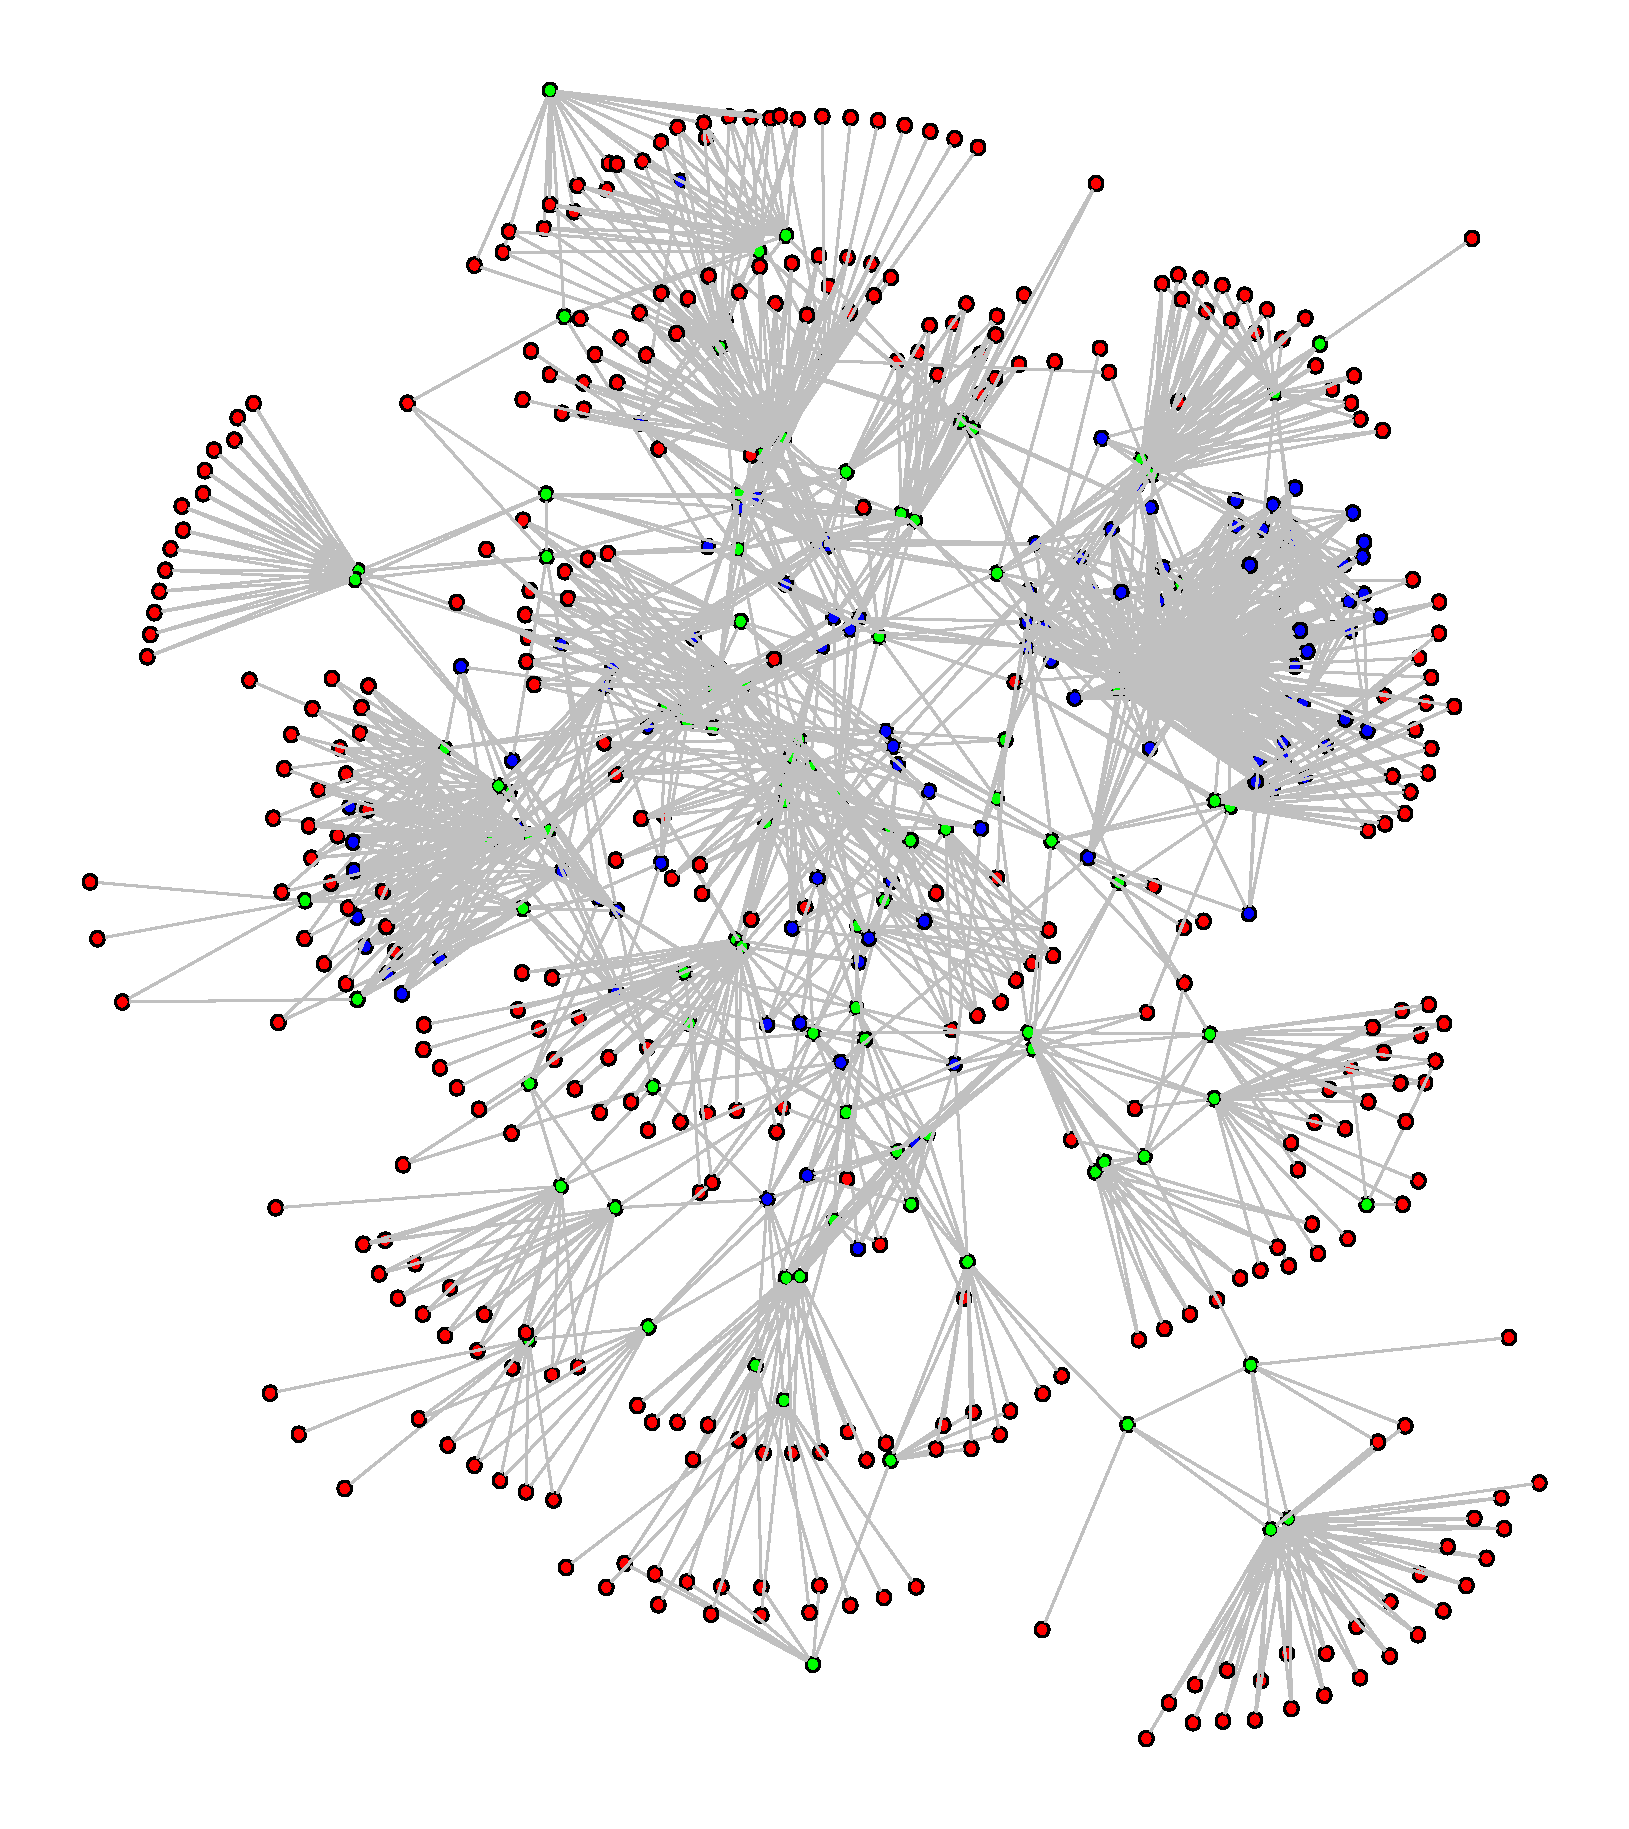
\includegraphics[scale=0.15,angle=90,height=3.5cm,width=8cm]{7018-r0}
  \vspace{-0.3cm}
  \caption{Internet-like topology: 344 client routers (red), 109 gateway routers (green), 109 backbone routers (blue)}\vspace{-.2cm}
  \label{fig:large-scale-topo}
\end{figure}

\begin{table}[htbp]
\centering
\caption{Large-scale topology link bandwidth and delay ranges}
\vspace{-0.3cm}
\label{tab:large-scale}
\begin{tabular}{|l||c|c||c|c|}
  \hline
  \multirow{2}{*}{\bf Link type} &  \multicolumn{2}{|c||}{\bf Delay} &  \multicolumn{2}{|c|}{\bf Bandwidth} \tabularnewline
  \cline{2-5}
                        &  Min & Max                       &  Min & Max \tabularnewline
  \hline \hline
  Backbone--Backbone    & 5~ms & 10~ms   & 40~Mbps & 100~Mbps \tabularnewline
  \hline
  Gateway--Backbone,    & \multirow{2}{*}{5~ms} & \multirow{2}{*}{10~ms}   
                        & \multirow{2}{*}{10~Mbps} & \multirow{2}{*}{20~Mbps} \tabularnewline
  Gateway--Gateway      & & & & \\
  \hline
  Client--Gateway       & 10~ms & 70~ms   & 1~Mbps  & 3~Mbps \\
  \hline
\end{tabular}
\vspace{-0.3cm}
\end{table}

%Priya: Leaving out this in the interest of space...
%Topological location of the data producer plays a key role in its resilience to Interest flooding attacks. For a data producer that %is connected to a client node via a low-bandwidth link, even a small number of junk Interests can impact services for legitimate %users. For a producer located at the backbone with rich connectivity through many high-bandwidth links, an attack might not %be as severe as a majority of legitimate users might not be on the attack path. 


% The results for all attack mitigation algorithms and all runs are aggregated in Fig.~\ref{fig:small-scale attack progress}, where Y-axis represents a minimum and maximum range for observed Interest satisfaction percentages among all nodes and all simulation runs.
% A short and simplistic summary of the results is that the first two attack mitigation methods do not work at all, and the last two are working quite good.

In Fig.~\ref{fig:large-scale}, we summarize our results aggregated over all simulations runs for each mitigation algorithm for the scenario where the data producer is placed at a gateway node. We observe similar results for the data producer placed at a backbone node as well. Unlike the binary-tree topology experiments, we observe that the satisfaction-based pushback is the most effective algorithm, while both the token bucket with per interface fairness and satisfaction-based Interest acceptance have poor performance.  Interest satisfaction percentage for legitimate users are close to 100\% and approximately 30\% and 25\% respectively for these mitigation methodologies.

%
%The evaluation results,\footnote{Note that for larger-scale experiments we reduced attack window to 15~minutes} summarized in Fig.~\ref{fig:large-scale}, show that performance of the token bucket with per interface fairness and satisfaction-based pushback algorithms are about at the same level as in small-scale evaluations (Fig.~\ref{fig:small-scale}), but with larger variations of minimum and maximum instantaneous satisfaction rates.

\begin{figure}[tbh]
 \centering
 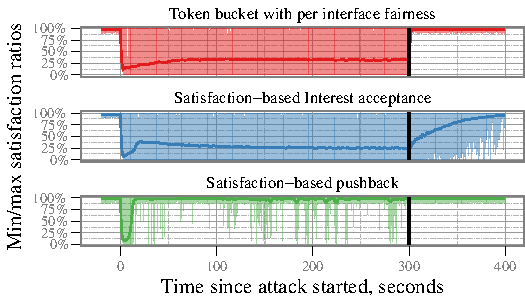
\includegraphics[scale=0.8]{paper-topo-7018-gw/7018-r0-good-0-producer-gw}
 \vspace{-.3cm}\caption{Satisfaction ratio dynamics during the attack for large-scale topology with 40\% attackers)}\vspace{-.3cm}
 % producer on a gateway node
 \label{fig:large-scale}
\end{figure}

Satisfaction-based Interest acceptance algorithm, which was very effective for binary-tree topology, is completely ineffective when deployed in a larger and more realistic topology.  For the duration of the attack, legitimate users experience poor quality of service with only 25\% of their Interests being satisfied and continue to experience degraded service long after the attack has stopped. This poor performance, as detailed in Section~\ref{sec:probabilistic}, is due to the fact that each router on the path makes an independent, uncoordinated decision on whether to forward or drop an Interest. In the case of the larger-topology, with much higher average hop count, Interest packets from legitimate users have a very low probability of reaching the data producer, resulting in poor Interest satisfaction statistics and further penalization of new Interests from them.

All our evaluations leave us to conclude that among the three techniques we tested under various topology and attacker concentrations, the satisfaction-based pushback is the most promising one in mitigating Interest flooding attacks.% and it restricts malicious Interests from even entering the network. 
%The only short periods of time when malicious Interests are getting admitted to the network is when routers have either no prior knowledge about per-interface satisfaction ratios (the initial period of the attack) or such knowledge becomes stale (statistics decaying during the attack). As soon as the knowledge is obtained or refreshed, the service for legitimate users returns to norm.


% Alex: Anything else here?

% Alex: I also experimented with placing producer at the backbone, getting slightly better results for all algorithms.  Though I'm not sure there is any value to put those results in the paper

% \subsection{Simulation versus Emulation}
\label{sec:simemu}
Before committing significant efforts into simulation-based implementation of designed defensive techniques it was necessary to confirm that ndnSIM has close performance characteristics to the reference NDN implementation - Project CCNx. This will guarantee that evaluation results derived from simulations will be meaningful in real NDN world.

To achieve this goal a comparison of Project CCNx software and ndnSIM software was performed under small scale Interest flooding attack. DETER Testbed was used as emulation tool for CCNx evaluation. Using it we were able to setup non-virtualized Ubuntu nodes running CCNx 0.6.0 software connected in a binary tree topology with 4 leaves and 1 root node. A number of applications running on top of CCNx have been developed, namely:
\begin{itemize}
\item{Producer application serves 1KB data packets under a known for the attacker name prefix}
\item{Legitimate client application requests 5KB of data per second from the producer}
\item{Attacker application tries to fill the channel of the producer by sending 500 Interest packets per second}
\end{itemize} 

In this emulation scenario producer application occupied a root node, legitimate clients occupied all even leaves and attacker applications were put on all odd leaves. With 100kb links with 40ms delay such setup leads to no congestion during the period when attackers are turned off and congestion when they are turned on (seconds 60-90). Exactly the same scenario was replicated for ndnSIM evaluation, however, we had to adjust the sending rate of attacker application in order to produce the same amount of congestion in the network. Sending rates are compared in Figure~\ref{fig:simemupower}. To achieve the identical slope and height of sending rate of evil Interests by attacker nodes we had to reduce sending rate of simulation-based attacker application by 30\%. The most likely reason for that is the overhead of Java virtual machine and operating system itself during the emulation of CCNx that results in eventual 30\% slower Interest transmission.  

Once we achieved the same characteristics of Interest flooding attack we were able to compare data packet losses by legitimate clients. Figure~\ref{fig:simemuperf} shows the cumulative received data by legitimate consumers in emulation and simulation experiments. NdnSIM performs worse due to its more deterministic nature, while the effects of UDP protocol usage, operating system process scheduling, and other kernel level operations on packet queues provide more randomness and a better intermixing of bad and good traffic which gives a slightly better performance. To summarize, we can use ndnSIM for our evaluations and real world performance is likely to be even better than our evaluation results.

\begin{figure}[htpb]
  \centering
  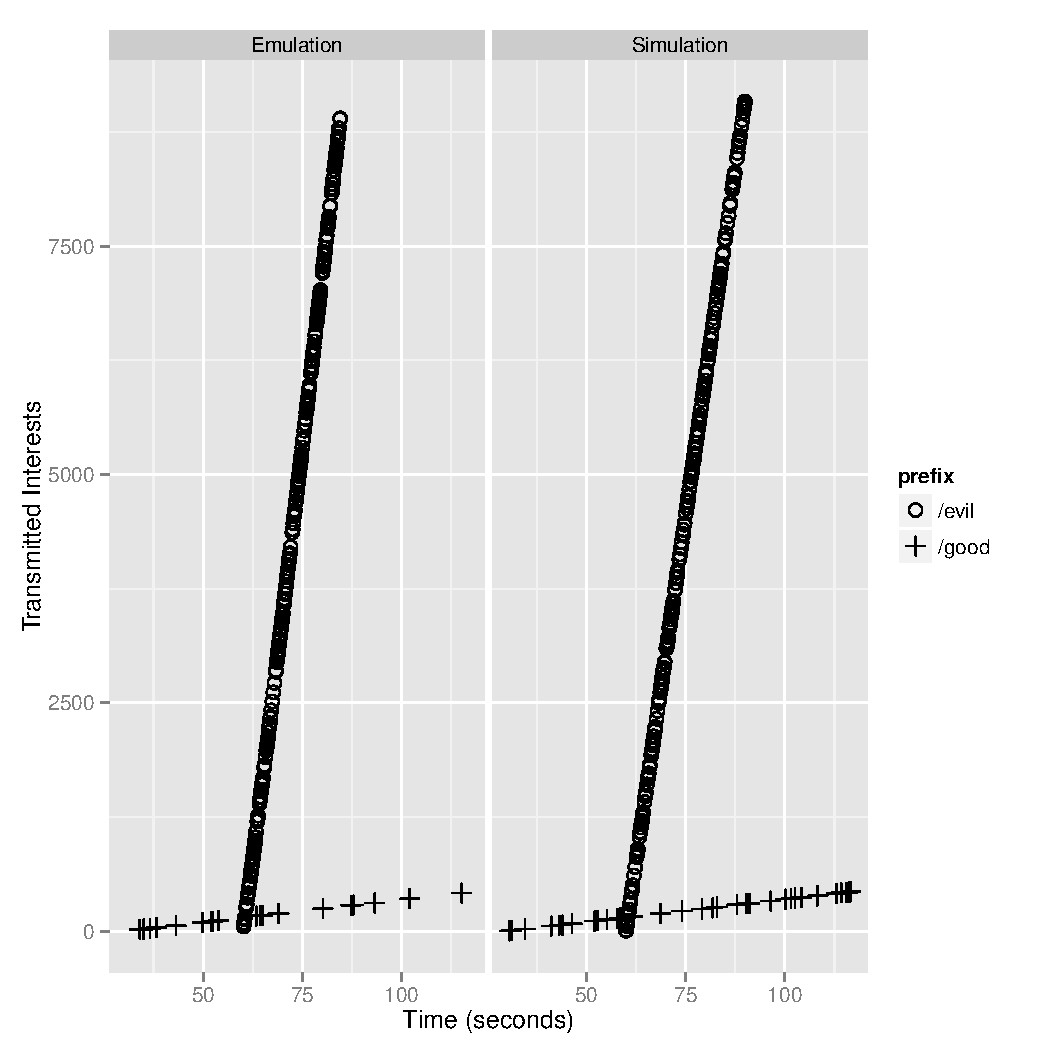
\includegraphics[scale=0.5]{figures/sim-emu-power.pdf}
  \caption{Strength of Interest flooding attack}
  \label{fig:simemupower}
\end{figure}

\begin{figure}[htpb]
  \centering
  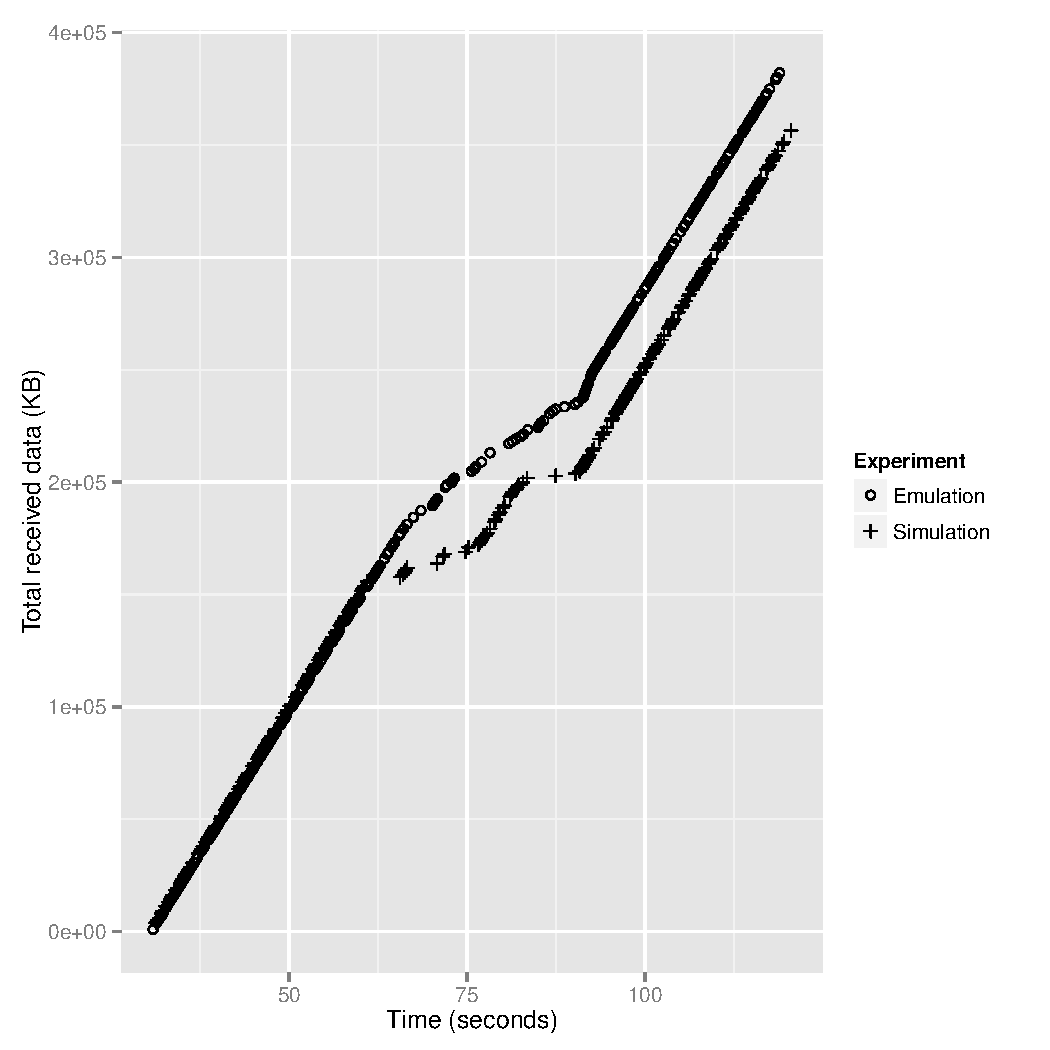
\includegraphics[scale=0.5]{figures/sim-emu-performance.pdf}
  \caption{Data retrieval by legitimate clients}
  \label{fig:simemuperf}
\end{figure}



\subsection{Limitations}
%{\color{red} I gave up the idea of seperate discussion section after trying for some time, as given the space limitation, there is no way to write a reasonably comprehensive and  broad discussion section that justifies a separate section. Instead, I decided to have a scoped down version here that confesses upon the limiations of our evaluations only. Whoever has time (I need to sleep few hours), please go ahead and write 1-2 paragraphs as I outlined below. -Ersin}

%This section should roughly say: Our results show that the two features, namely the symmetric traffic and stateful routing, give NDN routers the ability to observe and characterize traffic in real time. Through our evaluations, we demonstrated that a mitigation algorithm that leverages such ability has great potential in mitigating various DDoS attacks that could otherwise have grave effect on the network. However, as the first step in exploring the problem and the solution space, this paper has obvious limitations: (1) We assume a simple attacker model that would be most effective in vanilla NDN and keep it static during our evaluations. Although it is a valid and important step in showing the effectiveness of a particular mitigation approach, the next natural step is evaluating the above described solutions with more sophisticated and adaptive attackers. (2)   Although most (such as single-path routing, no-caches in the network, single homed victim, etc) are aimed to test the proposed solutions under worst-case scenario, we made many assumptions in simulations/evaluations about the configurations, topology and the traffic that maybe poor-representative of realistic conditions. (3) As NDN being an ongoing research effort itself, our evaluations fully depend on simulations and done over a snapshot of its codebase.       

% The main contribution of the paper and this section in particular is a proof that two inherent properties of NDN architecture, namely the symmetric traffic and stateful forwarding, give NDN routers the ability to characterize traffic and react in real time. 
% We demonstrated that satisfaction-based pushback algorithm, leveraging this ability, has great potential in mitigating various DDoS attacks that could otherwise have a grave effect on the network. 
% However, as the first step in exploring the problem and the solution space, our paper has obvious limitations.
% First, we assumed a simple attacker model that would be most effective in vanilla NDN and keep it static during our evaluations. 
% Although it is a valid and important step in showing the effectiveness of a particular mitigation approach, the next natural step that we are leaving out for future work is evaluating the above described solutions with more sophisticated and adaptive attackers. 
% Second, while aiming to test the designed algorithms under worst-case conditions, the future work needs to address behavior in more realistic scenarios, including investigation of multi-path routing, in network caches, as well as multi-homed victims.

This paper is a first step in understanding the impact of Interest flooding attacks in NDN and exploring the solution space. 
While designing our mitigation algorithms, we exploit two key features of NDN architecture, namely routers maintaining state about the Interests they have forwarded and Data traffic taking the reverse path of the Interest traffic. 
We test the efficacy of our algorithms by simulating them on both a simple binary-tree topology, % designed to test the worst-case effectiveness of our algorithms as well as on a realizing 
as well as a more realistic ISP-based topology designed to provide insights of our algorithms' behavior when deployed on a real network. 
While our results are promising and show a great potential in mitigating Interest flooding DDoS attacks, there are certain limitations which should be addressed in future research. 

First, in our evaluations we used a simple and static attacker model---attackers send junk Interests as fast as possible. 
In future work, we plan to explore the impact of models where the attackers are more sophisticated and dynamically adapt their behavior and Interest sending patterns based on the network reaction. 
Second, we assumed that Interests are not satisfied by an intermediate router's cache and always forwarded all the way to the producer.  
In future, we plan to study the impact of Interest flooding attacks in more realistic scenarios with multi-path routing enabled, more realistic traffic patterns, and the presence of in-network caches.
% We also ignored NDN's strategy layer that routes around failure and congestion in the network. 
% In future work, we plan to study the impact of turning on these features. 
%Finally, we also plan to perform more extensive simulations on other realistic Internet-like topologies and traffic patterns.



\section{Related work}
\label{sec:related-work}

As a new Internet architecture proposal, Named Data Networking has attracted attention from the security community. 
Lauinger~\cite{Lauinger:2010:Security--scalability} showed several possible attacks against some specific design choices implemented in CCNx software (\url{http://www.ccnx.org/}); in particular~\cite{Lauinger:2010:Security--scalability} explored the issue of user privacy, assuming users are concentrated on the same edge router only and one can obtain complete knowledge of cached content.  
W\"ahlisch et al.~\cite{Wahlisch:2012:Backscatter-from} explore security and stability threats in the general area of information-centric networks (ICN), using CCNx software as an example.  
While this work aims to generalize findings for all ICNs, it largely does not go beyond the current design choices of CCNx.
% (which is an example, but not the final word in NDN) 
% Gasti et al.~\cite{gasti2012ddos} identified several NDN architecture-specific attacks (Interest flooding and content/cache poisoning) and proposed potential solutions, without devising particular algorithms.
In this paper we follow the suggestions by Gasti et al.~\cite{gasti2012ddos} and utilize the properties provided by the NDN architecture to mitigate DDoS attacks, and tackle the Interest flooding problem as a first step in this direction.
More specifically our attack mitigation design relies on NDN's stateful forwarding plane that allows us to
maintain statistics on unsatisfied Interests.  
Similar approaches are also explored by Yi et al.~\cite{adaptive-forwarding,adaptive-tr} and Rozhnova et al.~\cite{rozhnova2012effective} to facilitate NDN network performance.

The general area of mitigating denial of service attacks is amongst the hottest topics in recent years.
% Among all the body of work, 
The most relevant works to this paper are the solutions to brute force IP packet flooding, such as DDoS detection techniques~\cite{Chen:2007:Collaborative-detection, Jun:2011:DDoS-flooding}, methods of pushing back malicious traffic to edges using various filtering techniques~\cite{Pushback, Tupakula:2003:A-practical-method, Argyraki:2005:Active-internet, Oikonomou:2006:A-framework-for-a-collaborative, Liu:2008:To-filter-or-to-authorize:, Chou:2009:Proactive-surge, Liu:2010:NetFence:-preventing}, 
overlay-based filtering~\cite{Stone:2000:CenterTrack:-An-IP-overlay, Keromytis:2004:SOS:-An-architecture, Kline:2011:Shield:-DoS-filtering}, 
various ticketing systems with conditional admission of traffic in to the network~\cite{Yaar:2004:SIFF:-A-stateless, Yang:2005:A-DoS-limiting-network, Wendlandt:2006:Fastpass:-Providing, Natu:2007:Fine-grained-capabilities, Portcullis, Capabilities},
and systems that attempt to use approximate IP traffic symmetry to estimate and filter out malicious traffic~\cite{Wang:2002:Detecting-SYN-flooding, Kreibich:2005:Using-packet, Mahimkar:2007:dFence:-Transparent}. 
Identifying malicious traffic requires establishing certain state at routers, and the above mentioned solutions differ in the specifics on what state to use and how to establish it.  By design NDN's forwarding plane keeps per packet state at every router, the finest granularity state to support any and all mitigation solutions---we simply take full advantage of this state to develop desired solutions.

% Our design for the Interest flooding attack mitigation borrows 

% This paper talks about attacks on content centric infrastructure (not specifically to NDN).
% \cite{Wahlisch:2012:Backscatter-from}



% % Collaborative detection of DDoS attacks over multiple network domains
% \cite{Chen:2007:Collaborative-detection} distributed change-point detection

% % DDoS flooding attack detection through a step-by-step investigation
% \cite{Jun:2011:DDoS-flooding}

% % A practical method to counteract denial of service attacks
% \cite{Tupakula:2003:A-practical-method}


% Alex: We should not include this reference for the review, but afterwards
% Previous work on DDoS and DoS~\cite{gasti2012ddos}






% Network level (Flooding)
% % 2002
% Pushback~\cite{Pushback} (hop-by-hop push back) aggregate- based congestion control/congestion signatures (e.g., per-destination), rate-limiting, explicit notification
% AITF~\cite{Argyraki:2005:Active-internet} (active filtering requests; path recording, last-point of trust detecting)?
% DefCOM \cite{Oikonomou:2006:A-framework-for-a-collaborative} Communication between src, core, and dst to provide collaborative defense. Dst raises alerts, src differentiate bad/good, packet tagging. Core rate-limit, congestion-aware re-tag. Traffic prioritization.
% StopIt \cite{Liu:2008:To-filter-or-to-authorize:} (filtering) tagging with passports, tagged prioritization, dst- invoked filter instantiation
% NetFence \cite{Liu:2010:NetFence:-preventing} congestion policing: fair queuing (one leaky bucket per {src,L}, L- bottleneck), secure "ticketing" with signals for AIMD to increase/decrease bandwidth allowance
% PSP \cite{Chou:2009:Proactive-surge} topology as origin-destination pairs, packet tagging, OD traffic isolation, sharing based on historic bandwidth demand


% SIFF~\cite{Yaar:2004:SIFF:-A-stateless} (time-based tickets, capabilities)
% TVA \cite{Yang:2005:A-DoS-limiting-network} like SIFF, traffic- based tickets, hierarchical per- AS, per-source fair queuing
% FastPass \cite{Wendlandt:2006:Fastpass:-Providing} (tokens: various puzzles, other methods) traffic authorization, routers verify and filter.
% \cite{Natu:2007:Fine-grained-capabilities} based on TVA/SIFF: specifies previously unspecified mechanisms to grant "tickets" for requesters, extends capabilities to include priorities, changing tickets to be only destination- dependent, not path dependent
% % LazySusan \cite{Crowcroft:2007:Lazy-Susan:} TR (latency-based proof of work--- computational puzzles)
% Portcullis \cite{Portcullis} Protecting connection setup with computational proof of work, tickets and traffic prioritization for the rest, per- computational fairness; DNS to disseminate puzzles
% There are many other puzzle- based schemes, on which Portcullis is based or which problems it solves



% PacketSymmetry \cite{Kreibich:2005:Using-packet} (leverages packet symmetry to detect and remove bad traffic) packet asymmetry - number of transmitted packets (tx) to received packets (rx); negative values when rx outweighs tx, positive values when tx outweighs rx, and zero in the case of perfectly balanced traffic)
% % Detecting SYN flooding attacks
% \cite{Wang:2002:Detecting-SYN-flooding} based on the protocol behavior of TCP SYN-FIN (RST) pairs, and is an instance of the Seqnential Change Point Detection
% dFence \cite{Mahimkar:2007:dFence:-Transparent} (middleboxes) TCP connection proxying, rate estimation and TCP/ACK modification
 

% Overlays:
% CenterTrack \cite{Stone:2000:CenterTrack:-An-IP-overlay} (overlay) reroute suspicious traffic to a special routers with diagnostic capabilities using an overlay
% SOS \cite{Keromytis:2004:SOS:-An-architecture}
% Shield \cite{Kline:2011:Shield:-DoS-filtering}



% NDN and other future information centric architectures were lacking any DDoS mitigation techniques, so we put efforts in understanding DDoS defensive systems, which were made for IP architecture, for the purpose of possible incorporation of them in NDN. In this section we will overview generic directions of DDoS mitigation designs and try to think about which tricks could be used in NDN.  
  
% Capability-based systems allow routers to negotiate, perform and enforce limitations on bandwidth consumption on router-to-router and router-to-client links. Usually such systems require an extensive trust infrastructure in order to validate secure keys used by routers and clients. This implies that each client must pass through an authentication process prior to using any bandwidth~\cite{Capabilities}. We believe that for NDN this method doesn't fit really well for the following reasons. First, this method is very questionable in terms of scalability and mobility support since it requires tight trust connections between routers and hosts. Thus, it neglects one of the main advantages (mobility) of NDN. Second, the design of trust infrastructure for NDN is not well defined yet, which means that we cannot really make assumptions in our design of mitigation techniques.

% Computation-based systems provide each client an access to the network resources only after performing a significant computations such as solving puzzles. Spending a huge amounts of computational resources can effectively slow down a flooding attack by the botnet, however it also creates additional computational burden for legitimate clients. One of the main difficulties in such systems is the question of puzzle dessimination. In ~\cite{Portcullis} authors suggested to propagate puzzles using DNS system. In NDN since routers have caching abilities, we can propagate puzzles just like a normal data packets, using Interest-Data exchange. Overall, this method looks interesting and deserves being investigated in a future work.

% Congestion control systems do per flow traffic analysis and drop of packets belonging to misbehaving flows. For instance, Random Early Detect (RED)~\cite{RED} identifies flows that do not comply with TCP-friendly end-to-end congestion control, and preferentially drop them. Such techniques, if largely deployed, could perform well, however, they cannot provide effective defense against non-greedy botnets that are creating a huge amount of low-bandwidth flows. Since NDN routers maintain a richer per-packet state, which translates into a better per-flow statistics, these techniques can become much more effective when applied to NDN.

% Push back systems are trying to detect bad and good traffic flows on each router, and once attack is detected by one of the routers, it starts a coordinated push back by downrating incoming flows with a bad traffic in order to provide more capacity for a good traffic. This process is reiterating downstream till it reaches edge routers, which are directly connected to attacking bot machines~\cite{Pushback}. In general this technique can be applied to NDN architecture thanks to its decentralized coordination of downrating bad traffic flows. Moreover, NDN provides better capabilities for accurate flow detection.

%were looking for getting accustomed 

\section{Conclusion}
\label{sec:conclusion}

% Main take out from the paper:  could be a problem, but problem is solvable.  
% One of the key components in the Named Data Networking architecture is its stateful data delivery model, which potentially can be abused by new types of denial of service attacks.
% However, one should not forget that the same stateful data delivery provides effective mechanisms to fight back against such attacks.

%In this paper we demonstrated that NDN architecture can be quite resilient against Interest flooding attacks, which aim to overwhelm network capacity as well as memory resources on NDN routers.
%The most effective of the designed algorithms---satisfaction-based pushback---almost completely eliminates the attack (or at least mitigates it to an acceptable ``fair'' level), leveraging two key aspects: Interest/Data path symmetry and full receiver-based traffic control.
%In particular, it measures how well Interests are getting satisfied (path symmetry) and uses these measurements to adjust how many Interests can be accepted from each individual interface (receiver-based control), effectively pushing the attack to the edges.
%
%Other forms of attack may require different mitigation mechanisms.  
%However, the granularity of the NDN state---per each Interest packet---is what giving NDN an opportunity to stand against existing and new forms of attacks.
%
%NDN is a new networking paradigm that shifts the emphasis from endpoints to addressing content directly, thereby enabling secure and efficient content distribution. 

NDN being a newly proposed future Internet architecture, it is important to address its resilience in face of DDoS attacks. As an initial step in understanding the DDoS threats in NDN, we first examined a specific instance of DDoS attacks namely Interest flooding and the severe service degradation such an attack may cause to legitimate users. We then leveraged the key features of the NDN architecture to design, develop, and evaluate three mitigation strategies.
We performed detailed simulations on a range of topologies to quantify the effectiveness of our algorithms.   
The most effective algorithm---satisfaction-based pushback---was successful in almost completely shutting down the attackers, so that they cause little or no service impact to legitimate users.

NDN's stateful forwarding plane enables a number of desired functions, such as loop-free, multipath data delivery, built-in multicast, scalable content delivery, effective flow balance (i.e., congestion avoidance), and robust recovery from network failures, that people have attempted to install in IP networks~\cite{adaptive-forwarding}. Although this useful per-packet state can be abused to launch attacks, the demonstrated success of satisfaction-based pushback algorithm serves as evidence that one can indeed utilize the per packet state built into each NDN router to enable effective DDoS mitigation as well.  


\bibliographystyle{IEEEtran}
\bibliography{references}


\end{document}
